\section{有序合并:动态输入数据识别介绍}
我们的下一个并行模式是有序合并操作,它采用两个排序列表并生成一个组合的排序列表。 
有序合并操作可以用作排序算法的构建块,我们将在第 13 章“排序”中看到。 有序合并操作也构成了现代map-reduce框架的基础。 
本章介绍了一种并行有序合并算法,其中每个线程的输入数据是动态确定的。 
数据访问的动态特性使得利用局部性和平铺技术来提高内存访问效率和性能变得具有挑战性。 
动态输入数据识别背后的原理也与许多其他重要计算相关,例如集合交集和集合并集。 
我们提出了日益复杂的缓冲区管理方案,以提高顺序合并和其他动态确定其输入数据的操作的内存访问效率。

\subsection{背景}
有序合并函数接受两个排序列表 A 和 B,并将它们合并为一个排序列表 C。在本章中,我们假设排序列表存储在数组中。 
我们进一步假设这样的数组中的每个元素都有一个键。 在键上定义了由 $\leq$ 表示的顺序关系。 
例如,键可以是简单的整数值,并且$\leq$可以被定义为这些整数值之间的常规小于或等于关系。 在最简单的情况下,元素仅由键组成。

假设我们有两个元素 $e_{1}$ 和 $e_{2}$,其键分别为 $k_{1}$ 和 $k_{2}$。 
在基于关系 $\leq$ 的排序列表中,如果 $e_{1}$ 出现在 $e_{2}$ 之前,则 $k_{1} \leq k_{2}$。 
基于排序关系 $R$ 的合并函数采用两个排序的输入数组 $\mathrm{A}$ 和 $\mathrm{B}$,
分别具有 $\mathrm{m}$ 和 $\mathrm{n}$ 元素 ,其中 $\mathrm{m}$ 和 $\mathrm{n}$ 不必相等。 
数组 A 和数组 B 都根据排序关系 $\mathrm{R}$ 进行排序。 
该函数生成一个输出排序数组 $\mathrm{C}$,其中包含 $\mathrm{m}+\mathrm{n}$ 元素。 
数组 $\mathrm{C}$ 由数组 $\mathrm{A}$ 和 $\mathrm{B}$ 中的所有输入元素组成,并按排序关系 $\mathrm{R}$ 排序。

\begin{figure}[H]
	\centering
	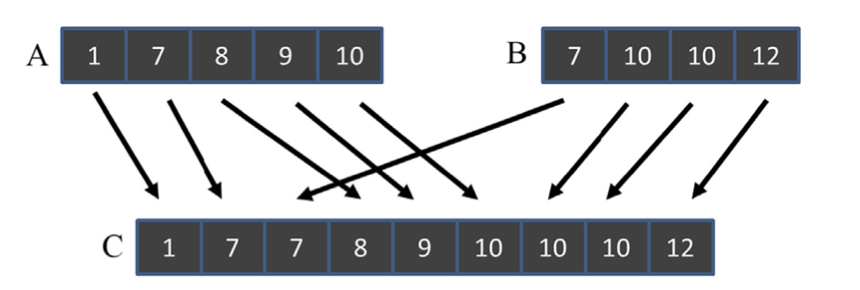
\includegraphics[width=0.9\textwidth]{figs/F12.1.png}
	\caption{\textit{合并算子的示例。}}
\end{figure}

图 12.1 显示了基于传统数字排序关系的简单合并函数的操作。 
数组 A 有五个元素 $(\mathrm{m}=5)$,数组 B 有四个元素 $(n=4)$。 
合并函数从 $A$ 和 $B$ 生成数组 $C$ 及其所有 9 个元素 $(m+n)$。 这些元素必须进行排序。 
图12.1中的箭头显示了如何将A和B的元素放入$\mathrm{C}$中以完成合并操作。 
每当 $\mathrm{A}$ 的元素和 B 的元素之间的数值相等时,A 的元素应该首先出现在输出列表 C 中。
此要求确保了有序合并操作的稳定性。

一般来说,如果具有相同键值的元素在输出中的放置顺序与它们在输入中出现的顺序相同,则排序操作是稳定的。 
图 12.1 中的示例演示了合并操作的输入列表和跨输入列表的稳定性。 
例如,将值为 10 的两个元素从 B 复制到 $\mathrm{C}$ 中,同时保持其原始顺序。 
这说明了合并操作的输入列表内的稳定性。 再例如,值为 7 的 A 元素在相同值的 $\mathrm{B}$ 元素之前进入 $\mathrm{C}$。 
这说明了合并操作的输入列表之间的稳定性。 稳定性属性允许排序操作保留当前排序操作中使用的键未捕获的先前排序。 
例如,列表 A 和 B 在按要用于合并的当前键排序之前可能已经根据不同的键排序。 
保持合并操作的稳定性允许合并操作保留前面步骤中完成的工作。

归并操作是归并排序的核心,归并排序是一种重要的可并行排序算法。 
正如我们将在第 13 章“排序”中看到的,并行合并排序函数将输入列表分为多个部分,并将它们分配给并行线程。 
线程对各个部分进行排序,然后协作合并排序后的部分。 这种分而治之的方法可以实现排序的高效并行化。

在现代 Map-Reduce 分布式计算框架(例如 Hadoop)中,计算被分发到大量计算节点。 
reduce过程将这些计算节点的结果组装成最终结果。 许多应用程序要求根据排序关系对结果进行排序。 
这些结果通常通过使用归约树模式中的合并操作来组装。 因此,高效的合并操作对于这些框架的效率至关重要。

\subsection{顺序合并算法}
\begin{figure}[H]
	\centering
	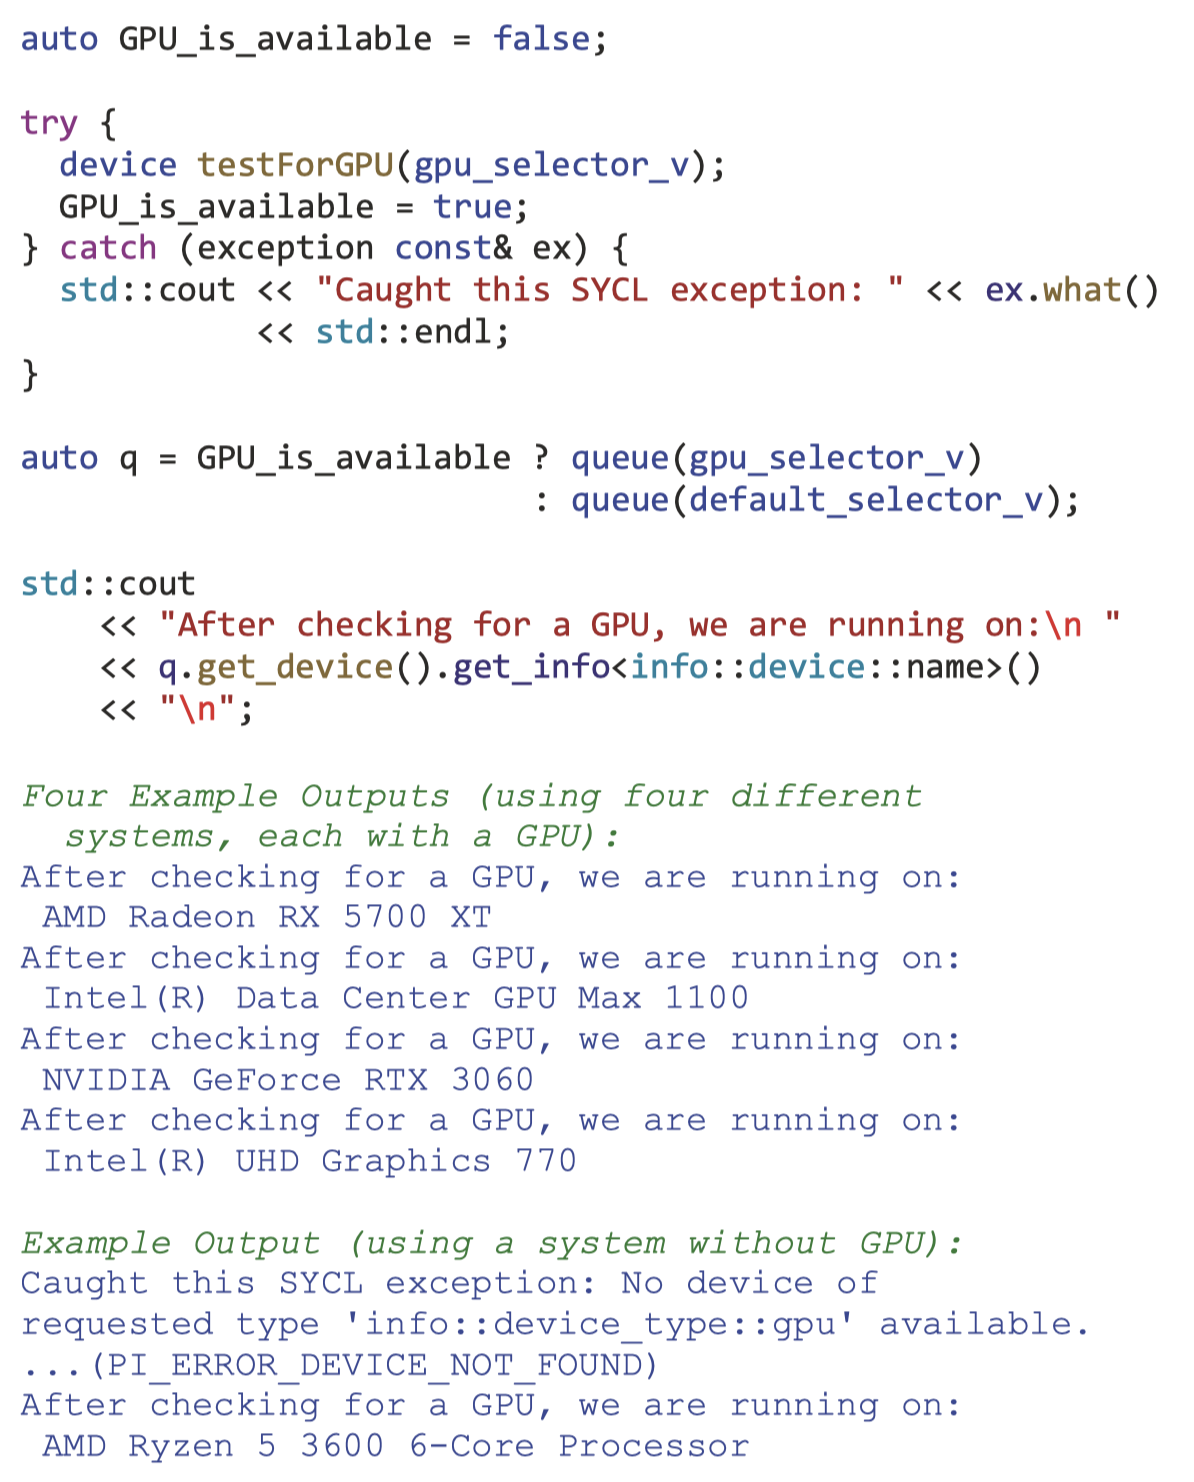
\includegraphics[width=0.9\textwidth]{figs/F12.2.png}
	\caption{\textit{顺序合并函数。}}
\end{figure}

合并操作可以使用简单的顺序算法来实现。 图 12.2 显示了顺序合并函数。

图 12.2 中的顺序函数由两个主要部分组成。 第一部分由一个 while 循环(第 05 行)组成,它按顺序访问 A 和 B 列表元素。 
循环从第一个元素开始:$\mathrm{A}[0]$ 和 $\mathrm{B}[0]$。 
每次迭代都会填充输出数组 C 中的一个位置; 将选择 A 的一个元素或 B 的一个元素作为该位置(第 06-10 行)。 
循环使用$\mathrm{i}$和$\mathrm{j}$来识别当前正在考虑的A和$\mathrm{B}$元素; 当执行第一次进入循环时,$i$和$j$都是0。 
循环进一步使用 $\mathrm{k}$ 来标识输出列表数组 $\mathrm{C}$ 中要填充的当前位置。 
在每次迭代中,如果元素$\mathrm{A}[\mathrm{i}]$小于或等于$\mathrm{B}[\mathrm{j}]$,
则$\mathrm{A}的值 [\mathrm{i}]$ 被分配给 $\mathrm{C}[\mathrm{k}]$。 
在这种情况下,执行会在进入下一次迭代之前递增 $\mathrm{i}$ 和 $\mathrm{k}$。 
否则,$B[j]$ 的值将赋给 $C[k]$。 在这种情况下,执行会在进入下一次迭代之前递增 $\mathrm{j}$ 和 $\mathrm{k}$。

当执行到达数组 A 的末尾或数组 B 的末尾时,执行将退出 while 循环。执行继续到第二部分,如图 12.2 右侧所示。 
如果数组 $\mathrm{A}$ 是已被完全访问过的数组(如 $\mathrm{i}$ 等于 $\mathrm{m}$ 这一事实所示),
则代码将复制数组的剩余元素 数组 B 到数组 C 的剩余位置(第 13-15 行)。 
否则,数组 B 就是被完全访问过的数组,因此代码将 A 的剩余元素复制到 C 的剩余位置(第 17-19 行)。 
请注意,为了保证正确性,if-else 结构是不必要的。 
我们可以简单地让两个 while 循环(第 13-15 行和 17-19 行)跟在第一个 while 循环后面。 
仅进入两个 while 循环中的一个,具体取决于 A 或 B 是否被第一个 while 循环耗尽。 
然而,我们包含了 if-else 结构,以使代码对读者来说更加直观。

我们可以使用图 12.1 中的简单示例来说明顺序合并函数的操作。 
在 while 循环的前三个 $(0-2)$ 迭代中,$\mathrm{A}[0]、\mathrm{A}[1]$ 和 $\mathrm{B}[0]$ 被分配给 分别为$\mathrm{C}[0]、\mathrm{C}[1]$和$\mathrm{C}[2]$。 执行将持续到迭代 5 结束。 
至此,列表$\mathrm{A}$被完全访问,执行退出while循环。 
$\mathrm{A}[0]$ 到 $\mathrm{A}[4]$ 和 $\mathrm{B}[0]$ 总共填补了六个 $\mathrm{C}$ 职位。 
if 构造的 true 分支中的循环用于将剩余的 B 元素(即 B[1] 到 $\mathrm{B}$ [3])复制到剩余的 $\mathrm{C}$ 位置。

顺序合并函数访问 $\mathrm{A}$ 和 $\mathrm{B}$ 中的每个输入元素一次,并写入每个 $C$ 位置一次。 
其算法复杂度为$\mathrm{O}(\mathrm{m}+\mathrm{n})$,其执行时间与要合并的元素总数成线性正比。

\subsection{并行化方法}
Siebert 和 Traff (2012) 提出了一种并行化合并操作的方法。 
在他们的方法中,每个线程首先确定它将产生的输出位置范围(输出范围),并使用该输出范围作为 co-rank 函数的输入,
以识别将被合并以产生 输出范围。 一旦确定了输入和输出范围,每个线程就可以独立访问其两个输入子数组和一个输出子数组。 
这种独立性允许每个线程对其子数组执行顺序合并函数,以并行进行合并。 
应该清楚的是,所提出的并行化方法的关键是联合排序函数。 我们现在将制定联合秩函数。

令 $\mathrm{A}$ 和 $\mathrm{B}$ 为两个输入数组,分别具有 $\mathrm{m}$ 和 $\mathrm{n}$ 元素。 
我们假设两个输入数组都根据排序关系排序。 每个数组的索引从 0 开始。 
令 $\mathrm{C}$ 为通过合并 $\mathrm{A}$ 和 $\mathrm{B}$ 生成的排序输出数组。 
显然,$\mathrm{C}$ 有 $\mathrm{m}+\mathrm{n}$ 个元素。 我们可以做出以下观察:

\begin{Observation}
对于任何 $\mathrm{k}$ 使得 $0 \leq \mathrm{k}<\mathrm{m}+\mathrm{n}$,
存在(情况 1)一个 $\mathrm{i} $ 使得 $0 \leq \mathrm{i}<\mathrm{m}$ 
和 $\mathrm{C}[\mathrm{k}]$ 从 $\mathrm{A}[\mathrm{i}]$ 接收其值
或(情况 2 )$\mathrm{j}$,在合并过程中使得 $0 \leq \mathrm{j}<\mathrm{n}$ 
和 $\mathrm{C}[\mathrm{k}]$ 接收其值 $\mathrm{B}[\mathrm{j}]$。
\end{Observation}

\begin{figure}[H]
	\centering
	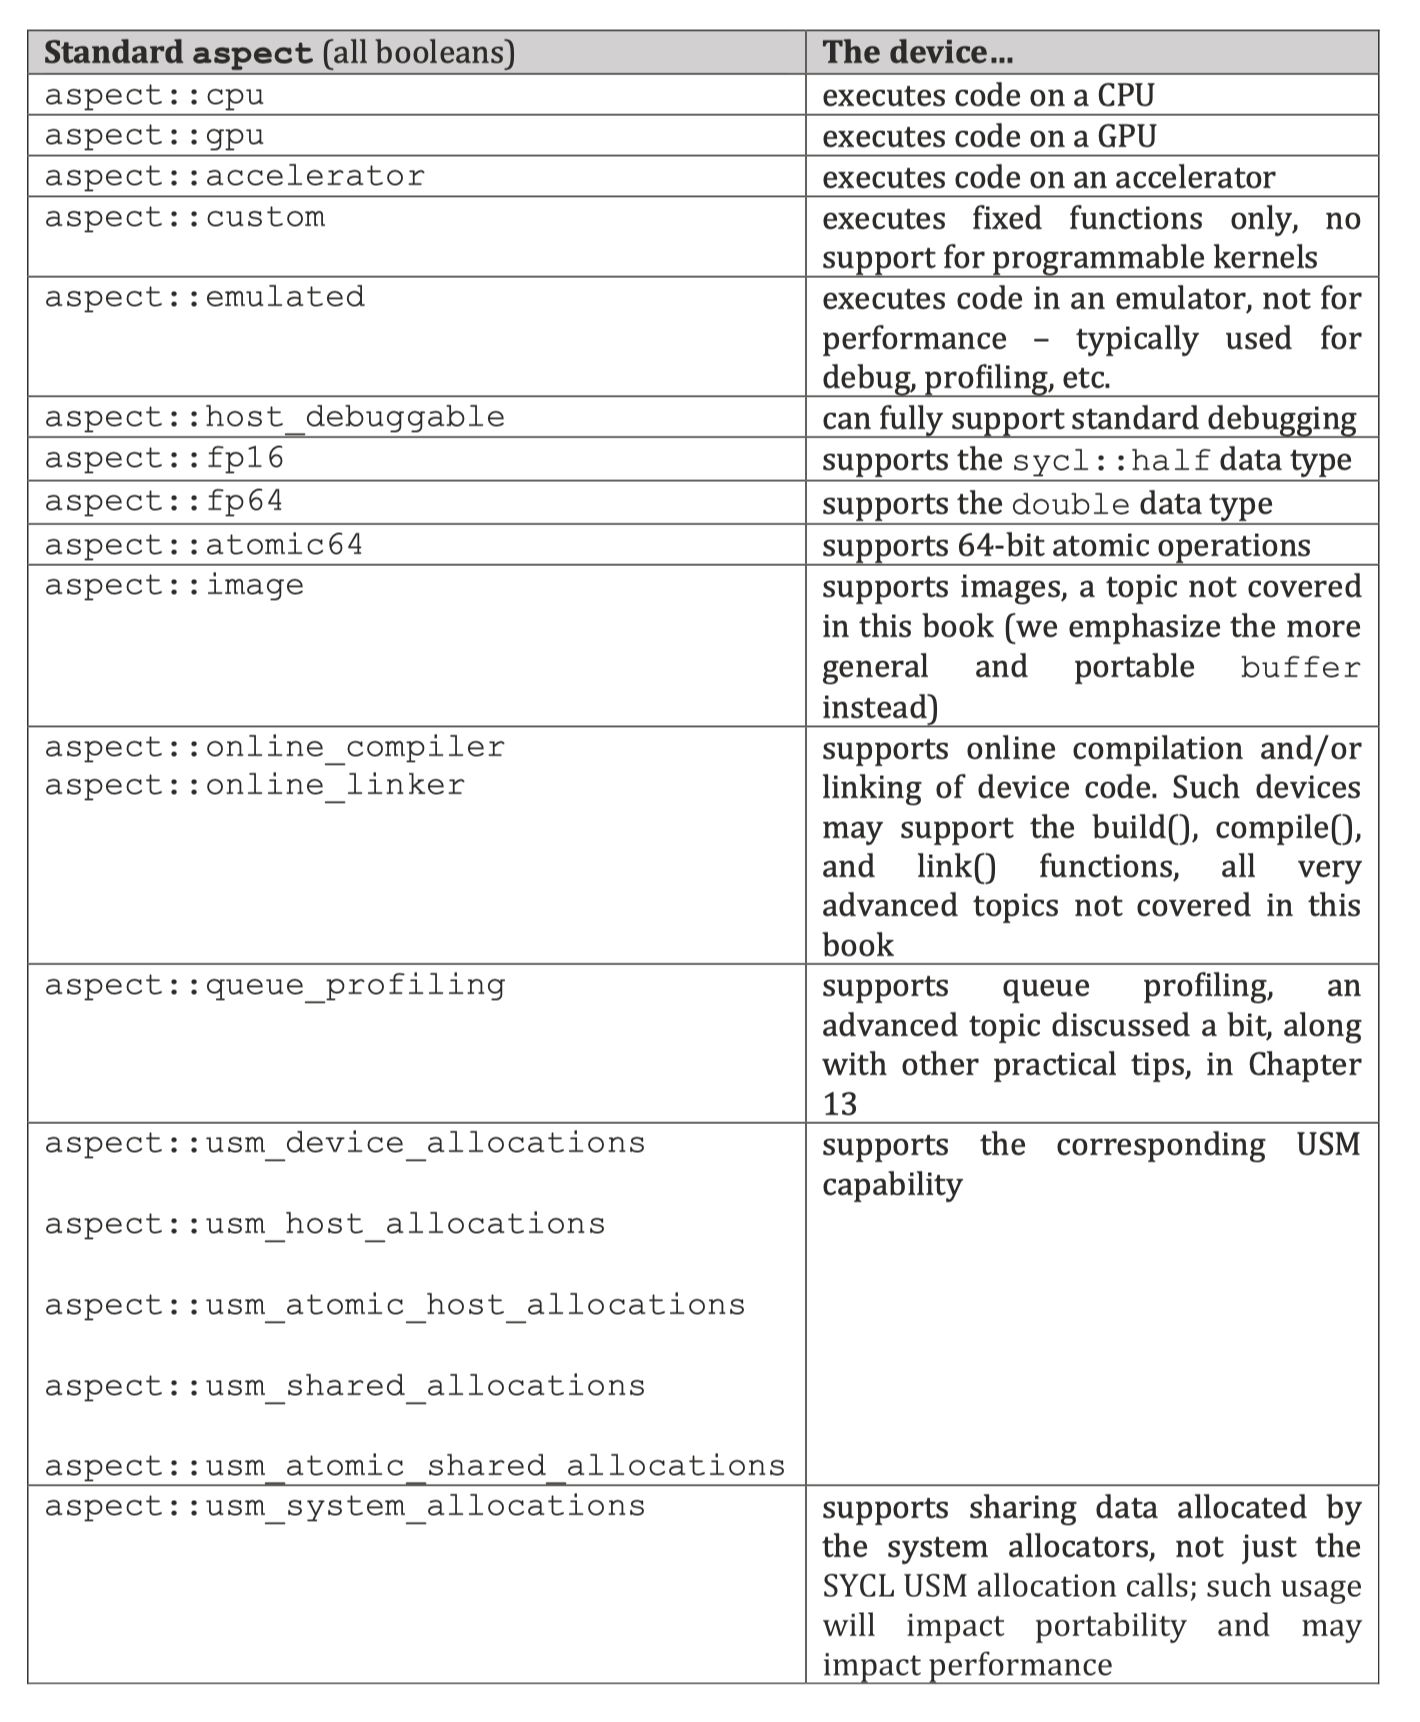
\includegraphics[width=0.9\textwidth]{figs/F12.3.png}
	\caption{\textit{观察实例1。}}
\end{figure}

图 12.3 显示了观察结果 1 的两种情况。 在第一种情况下,所涉及的 $\mathrm{C}$ 元素来自数组 A。
例如,在图 12.3A 中,C[4](值 9)从 $\mathrm{A}[3]$ 接收其值。 
在这种情况下,$\mathrm{k}=4$并且$\mathrm{i}=3$。 
我们可以看到$\mathrm{C}[4]$($\mathrm{C}[4]$ 之前的四个元素的子数组)的前缀子数组$\mathrm{C}[0]-\mathrm{C}[3]$, 
是 $A[3]$ 的前缀子数组 $A[0]-A[2]$($\mathrm{A}[3]$ 之前的三个元素的子数组)
和 $\mathrm{B}[1]$ 的前缀子数组 $\mathrm{B}[0]$ ($4-3=1$ 元素位于 $\mathrm{B}[1]$ 之前的子数组) 合并的结果。 
通式是子数组$\mathrm{C}[0]-\mathrm{C}[\mathrm{k}-1]$(k个元素)
是$\mathrm{A}[0]-\mathrm{A}[\mathrm{i}-1]$(i 个元素)
和 $\mathrm{B}[0]-\mathrm{B}[\mathrm{k}-\mathrm{i}-1] (\mathrm{k}-\mathrm{i}$ 元素)合并的结果。

在第二种情况下,所讨论的 $\mathrm{C}$ 元素来自数组 B。例如,在图 12.3B 中,C[6] 从 $B[1]$ 接收其值。 
在这种情况下,$k=6$并且$j=1$。 $\mathrm{C}[6]$ 的前缀子数组 $\mathrm{C}[0]-\mathrm{C}[5]$ 
($\mathrm{C}[6]$ 之前的六个元素的子数组) 是前缀子数组 $\mathrm{A}[0]-\mathrm{A}[4]$ 
($\mathrm{A}[5]$ 之前的五个元素的子数组)和$\mathrm{B}[0]$($B[1]$之前的 1 个元素的子数组)合并的结果。 
这种情况的一般公式是子数组 $C[0]-C[k-1](k$ elements) 是合并 $\mathrm{A}[0]-\mathrm{A}[\mathrm{ k}-\mathrm{j}-1](\mathrm{k}-\mathrm{j}$ 元素) 和 $\mathrm{B}$ $[0]-B[j-1]$ ( $j$ 元素)的结果。

在第一种情况下,我们找到$\mathrm{i}$并将$\mathrm{j}$导出为$\mathrm{k}-\mathrm{i}$。 
在第二种情况下,我们找到$\mathrm{j}$并将$\mathrm{i}$导出为$\mathrm{k}-\mathrm{j}$。 
我们可以利用对称性并将这两种情况总结为一个观察结果:

\begin{Observation}
对于任何$\mathrm{k}$,使得$0 \leq \mathrm{k}<\mathrm{m}+\mathrm{n}$,
我们可以找到$\mathrm{i}$和$\mathrm {j}$ 
使得 $\mathrm{k}=\mathrm{i}+\mathrm{j}, 0 \leq \mathrm{i}<\mathrm{m}$ 
和 $0 \leq \mathrm {j}<\mathrm{n}$, 
子数组 C[0]−C[k - 1] 是子数组 A[0]−A[i - 1] 和子数组 B[0]−B[j - 1] 合并的结果。.
\end{Observation}

Siebert 和 Traff (2012) 还证明了 i 和 j 是唯一的,
它们定义了生成长度为 k 的 C 的前缀子数组所需的 A 和 B 的前缀子数组。 对于元素 C[k],索引 k 称为其等级。 
唯一索引 i 和 j 被称为其联合秩。 例如,在图12.3A中,C[4]的秩和联合秩是4、3和1。再例如,C[6]的秩和联合秩是6、5和1。

共同排序的概念为我们提供了并行化合并函数的途径。 
我们可以通过将输出数组划分为子数组并将一个子数组的生成分配给每个线程来在线程之间划分工作。 
一旦完成分配,每个线程要生成的输出元素的等级就已知。 
然后,每个线程使用 co-rank 函数来确定需要合并到其输出子数组中的两个输入子数组。

请注意,合并函数的并行化与我们之前所有模式的并行化之间的主要区别在于,每个线程要使用的输入数据的范围无法通过简单的索引计算来确定。 每个线程要使用的输入元素的范围取决于实际的输入值。 这使得并行合并操作成为一种有趣且具有挑战性的并行计算模式。

\subsection{联合秩函数实现}
我们将 co-rank 函数定义为一个函数,它采用输出数组 C 中元素的秩 (k) 以及有关两个输入数组 A 和 B 的信息,
并返回 输入数组 A。 co-rank 函数具有以下签名:

\begin{figure}[H]
	\centering
	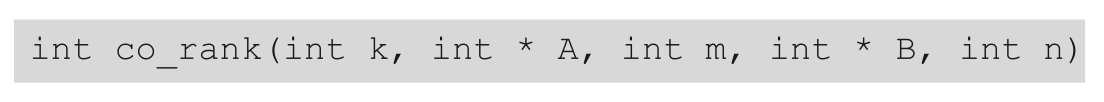
\includegraphics[width=0.9\textwidth]{figs/F12-a1.png}
\end{figure}

其中 $\mathrm{k}$ 是相关 $\mathrm{C}$ 元素的秩,$\mathrm{A}$ 是指向输入 $\mathrm{A}$ 数组的指针,
$\mathrm{ m}$ 是 $\mathrm{A}$ 数组的大小,$\mathrm{B}$ 是指向输入 $\mathrm{B}$ 数组的指针,
$\mathrm{n}$ 是 输入B数组,返回值是$\mathrm{i}$,即$\mathrm{k}$在A中的co-rank。
然后调用者可以导出 j,即 B 中 k 的联合秩,作为 k - i。

\begin{figure}[H]
	\centering
	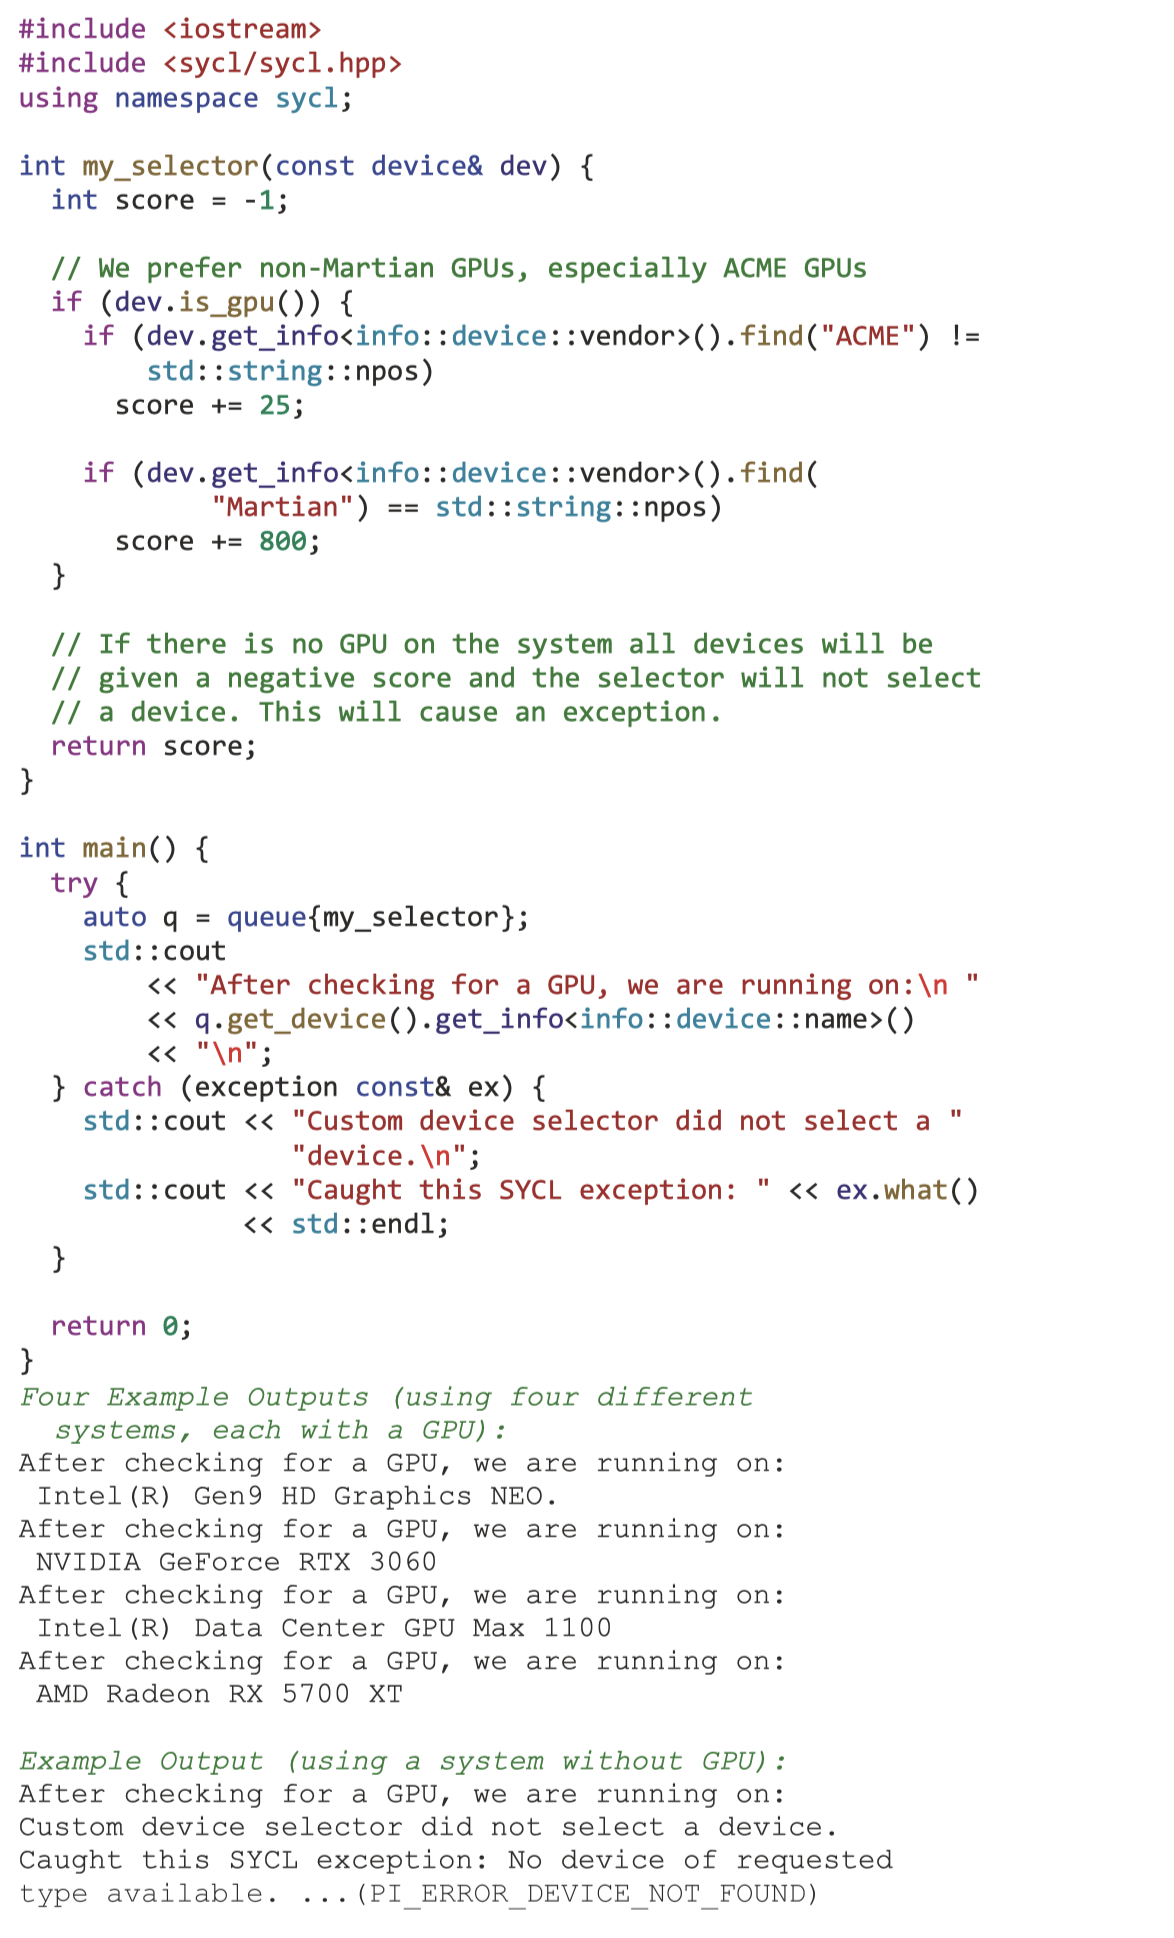
\includegraphics[width=0.9\textwidth]{figs/F12.4.png}
	\caption{\textit{联合排序函数执行示例。}}
\end{figure}

在我们研究 co-rank 函数的实现细节之前,首先了解并行合并函数使用它的方式是有益的。 
co-rank 函数的这种使用如图 12.4 所示,其中我们使用两个线程来执行合并操作。 
我们假设线程 0 生成 $\mathrm{C}$ $[0]-\mathrm{C}[3]$,线程 1 生成 $\mathrm{C}[4]-\mathrm{C}[8]$ 。

直观上,每个线程调用 co-rank 函数来导出 $\mathrm{A}$ 和 $\mathrm{B}$ 子数组的起始位置,
这些子数组将合并到 $\mathrm{C}$ 子数组中,即 分配给线程。 例如,线程 1 使用参数 (4, A, 5, B, 4) 调用 co-rank 函数。 
线程 1 的联合秩函数的目标是为其秩值 $k 1=4$ 识别联合秩值 $i 1=3$ 和 $j 1=1$。 
也就是说,从 $\mathrm{C}[4]$ 开始的子数组是通过合并从 $\mathrm{A}$ [3] 和 B[1] 开始的子数组生成的。 
直观上,我们正在从 A 和 $B$ 中查找总共四个元素,这些元素将在线程 1 合并其元素之前填充输出数组的前四个元素。 
通过目视检查,我们发现 $i 1=3$ 和 $\mathrm{j} 1=1$ 的选择满足我们的需求。 
线程 0 将采用 $\mathrm{A}[0]-\mathrm{A}[2]$ 和 $\mathrm{B}[0]$,
忽略 $\mathrm{A}[3]$ (值 9 ) 和 $\mathrm{B}[1]$ (值 10),这是线程 1 将开始合并的位置。

如果我们将 $i 1$ 的值更改为 2 ,我们需要将 $\mathrm{j} 1$ 值设置为 2 ,
这样我们仍然可以在线程 1 之前拥有总共四个元素。 然而,这意味着我们将在线程 0 的元素中包含值为 10 的 B[1]。 
该值大于线程 1 的元素中包含的 $\mathrm{A}[2]$ (值 8)。 这样的更改会导致生成的 $\mathrm{C}$ 数组无法正确排序。 
另一方面,如果我们将 i1 的值更改为 4 ,则需要将 j1 值设置为 0 以保持元素总数为 4 。 
但是,这意味着我们在线程 0 的元素中包含 $A[3]$(值 9),该元素大于 B[0](值 7),
而 B[0] 将被错误地包含在线程 1 的元素中。 这两个例子表明搜索算法可以快速识别值。

除了识别其输入段的开始位置之外,线程 1 还需要识别它们的结束位置。 
为此,线程 1 还调用参数为 $(9$, A, 5, B, 4) 的 co-rank 函数。 
从图 12.4 中我们看到 co-rank 函数应该产生 co-rank 值 $\mathrm{i} 2=5$ 和 $\mathrm{j} 2=4$。 
也就是说,由于 $\mathrm{C}[9]$ 超出了 $\mathrm{C}$ 数组的最后一个元素,
因此 $\mathrm{A}$ 和 $\mathrm{B}$ 数组的所有元素 如果试图生成从 $C[9]$ 开始的 $C$ 子数组,应该已经耗尽了。 
一般来说,线程 t 使用的输入子数组由线程 t 和线程 t + 1 的共同排序值定义:
$\mathrm{A}\left[ \mathrm{i}_{\mathrm{t}}\right]-\mathrm{A}\left[\mathrm{i}_{\mathrm{t}+1}\right]$ 
和 $\mathrm{B }\left[\mathrm{j}_{\mathrm{t}}\right]-\mathrm{B}\left[\mathrm{j}_{\mathrm{t}+1}\right]$。

\begin{figure}[H]
	\centering
	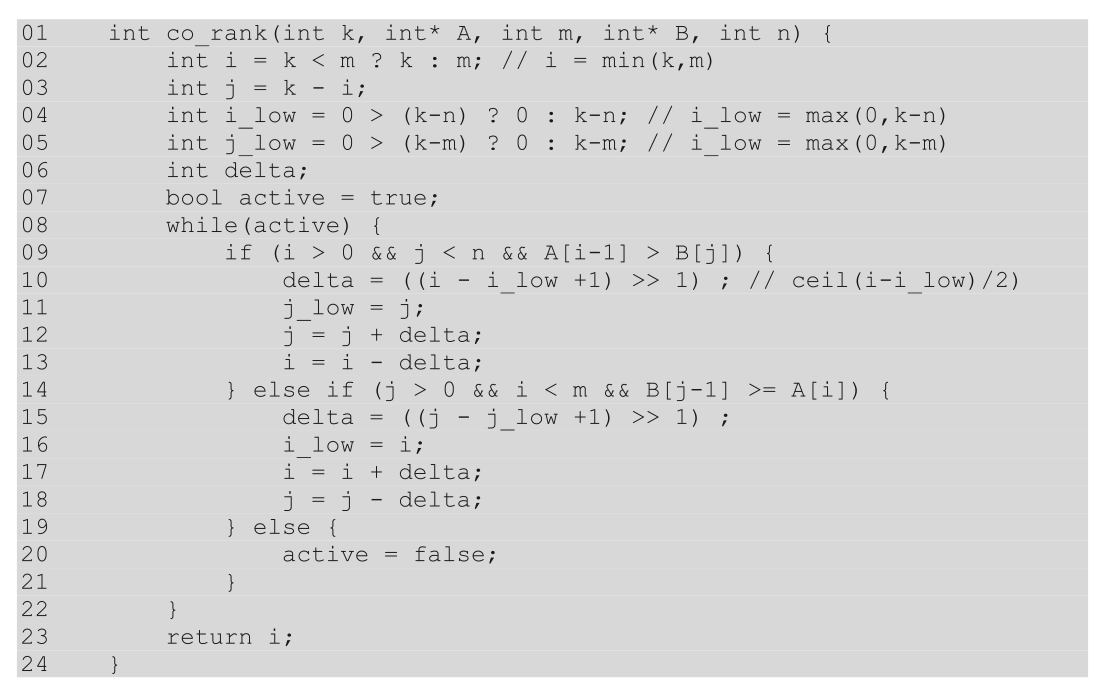
\includegraphics[width=0.9\textwidth]{figs/F12.5.png}
	\caption{\textit{基于二分搜索的联合排名函数。}}
\end{figure}

co-rank 函数本质上是一种搜索操作。 
由于两个输入数组都已排序,因此我们可以使用二分搜索甚至更高的基数搜索来实现搜索的计算复杂度 $\mathrm{O}(\log \mathrm{N})$。 图 12.5 显示了基于二分搜索的联合排序函数。 
co-rank 函数使用两对标记变量来描绘 $\mathrm{A}$ 数组索引的范围以及考虑用于 co-rank 值的 $\mathrm{B}$ 数组索引的范围。 变量 $i$ 和 $j$ 是当前二分搜索迭代中正在考虑的候选联合秩返回值。 
变量 i\_low 和 $j_{-}$low 是函数可以生成的最小可能的联合秩值。 
第 02 行将 $i$ 初始化为其最大可能值。如果 $\mathrm{k}$ 值大于 $\mathrm{m}$,
则第 02 行将 $\mathrm{i}$ 初始化为 $\mathrm{m}$,因为 co-rank $i$ 值不能 大于 A 数组的大小。 
否则,第 02 行将 $\mathrm{i}$ 初始化为 $\mathrm{k}$,因为 $\mathrm{i}$ 不能大于 $\mathrm{k}$。 
联合秩 $\mathrm{j}$ 值被初始化为 $\mathrm{k}-\mathrm{i}$ (第 03 行)。 
在整个执行过程中,co-rank 函数保持着这种重要的不变关系。 
$\mathrm{i}$ 和 $\mathrm{j}$ 变量的总和始终等于输入变量 $\mathrm{k}$ 的值(秩值)。

i\_low 和 j\_low 变量的初始化(第 4 行和第 5 行)需要更多解释。 
这些变量使我们能够限制搜索范围并使其更快。 从功能上讲,我们可以将这两个值设置为零,并让其余的执行将它们提升到更准确的值。 
当 $\mathrm{k}$ 值小于 $\mathrm{m}$ 和 $\mathrm{n}$ 时,这是有意义的。 
然而,当$\mathrm{k}$大于$\mathrm{n}$时,我们知道$\mathrm{i}$值不能小于$\mathrm{k}-\mathrm{n}$ 。 
原因是 B 数组中可以出现的 $\mathrm{C}[\mathrm{k}]$ 前缀子数组元素的最大数量为 $\mathrm{n}$。 
因此,至少有 $\mathrm{k}-\mathrm{n}$ 个元素必须来自 $\mathrm{A}$。 
因此$\mathrm{i}$值永远不会小于$\mathrm{k}-\mathrm{n}$; 
我们也可以将 i\_low 设置为 $\mathrm{k}-\mathrm{n}$。 
同样的道理,$\mathrm{j}_{-}$low 值不能小于 $\mathrm{k}-\mathrm{m}$,即 $\mathrm{B 的元素个数最少 }$ 必须在合并过程中使用,因此是最终联合秩 $\mathrm{j}$ 值的下限。

\begin{figure}[H]
	\centering
	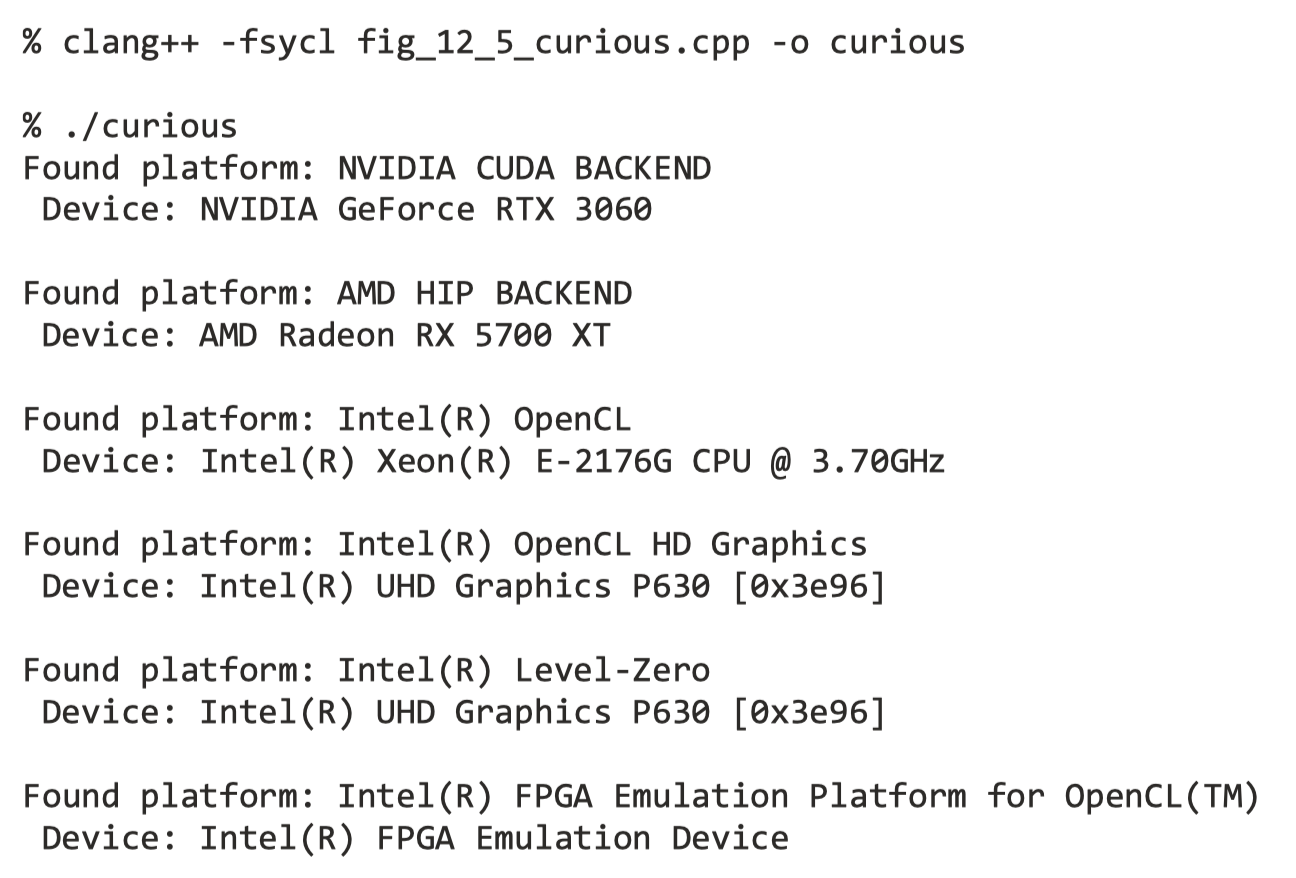
\includegraphics[width=0.9\textwidth]{figs/F12.6.png}
	\caption{\textit{线程 1 的 co-rank 函数操作示例的迭代 0。}}
\end{figure}

我们将使用图12.6中的示例来说明图12.5中的co-rank函数的操作。 
该示例假设使用三个线程将数组 $\mathrm{A}$ 和 $\mathrm{B}$ 合并到 $\mathrm{C}$ 中。 
每个线程负责生成包含三个元素的输出子数组。 
我们将首先跟踪线程 1 的 co-rank 函数的二分搜索步骤,该函数负责生成 $C[3]-C[5]$。 
读者应该能够确定线程 1 使用参数 (3, A, 5, B, 4) 调用 co-rank 函数。

如图 12.5 所示,co-rank 函数的第 2 行将 $i$ 初始化为 3,即 $\mathrm{k}$ 值,
因为 $\mathrm{k}$ 小于 $\mathrm{ m}$(值 5)在此示例中。 另外, i\_low 设置为 0 。 
$\mathrm{i}$ 和 i\_low 值定义当前正在搜索以确定最终联合秩 $i$ 值的 A 数组部分。 
因此,只有 $0,1,2$ 和 3 被考虑作为共同秩 i 值。 类似地, $\mathrm{j}$ 和 j\_low 值设置为 0 和 0 。

co-rank 函数的主体是一个 while 循环(第 08 行),它迭代地放大最终的 co-rank $i$ 和 $j$ 值。 
目标是找到一对 $i$ 和 $j$ 值,得到 $\mathrm{A}[\mathrm{i}-1] \leq \mathrm{B}[\mathrm{j}]$ 
和 $\mathrm{B}[\mathrm{j}-1]<\mathrm{A}[\mathrm{i}]$。 
直觉是,我们选择 $\mathrm{i}$ 和 $\mathrm{j}$ 值,
因此用于生成前一个输出子数组(称为前一个 A 子数组)的 A 子数组中的任何值都不应该是 大于用于生成当前输出子数组(称为当前B子数组)的B子数组中的任何元素。 
请注意,前一个子数组中的最大 A 元素可能等于当前 B 子数组中的最小元素,
因为只要 A 元素和 B 元素之间出现平局,A 元素就会优先放置到输出数组中,因为 稳定性要求。

在图 12.5 中,while 循环中的第一个 if 结构(第 09 行)测试当前 $i$ 值是否太高。 
如果是这样,它将调整标记值,以便将 $i$ 的搜索范围向较小的一端减少大约一半。 
这是通过将 i 值减少 $i$ 和 i\_low 之间差异的大约一半来完成的。 
在图 12.7 中,对于 while 循环的迭代 0,if 结构发现 i 值 (3) 太高,因为值为 8 的 A[i$1]$ 大于 $B[j ]$,其值为 7 。 
接下来的几条语句继续通过将 i 的值减少 delta $=(3-0+1)$ $\gg 1=2$ (第 10 和 13 行)来减少 i 的搜索范围,
同时保持 i\_low 值不变。 因此,下一次迭代的 i\_low 和 $i$ 值将是 0 和 1 。

该代码还通过将 $j$ 的搜索范围移动到当前 $j$ 位置之上,使其与 $i$ 的搜索范围相当。 
此调整保持了 $\mathrm{i}$ 和 $\mathrm{j}$ 之和应等于 $\mathrm{k}$ 的属性。 
通过将当前 $\mathrm{j}$ 值分配给 $\mathrm{j}_{-}$low (第 11 行)并将增量值添加到 $\mathrm{j}$ (第 12 行)来完成调整 。 在我们的示例中,下一次迭代的 $j_{-}$low 和 $\mathrm{j}$ 值将为 0 和 2 。

\begin{figure}[H]
	\centering
	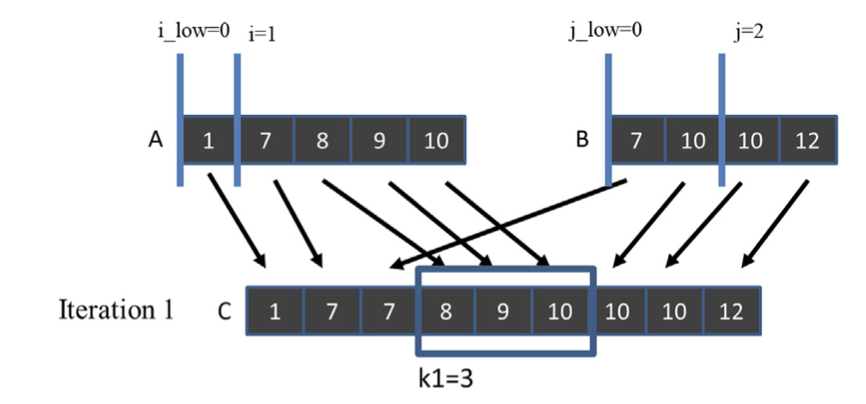
\includegraphics[width=0.9\textwidth]{figs/F12.7.png}
	\caption{\textit{线程 1 的 co-rank 函数操作示例的迭代 1。}}
\end{figure}

在 while 循环的第 1 次迭代期间,如图 12.7 所示,$i$ 和 $j$ 值为 1 和 2。
if 结构(第 9 行)发现 $\mathrm{i}$ 值是可接受的 因为 $\mathrm{A}[\mathrm{i}$ - 1] 是 $A[0]$ ,其值为 1 ,
而 $B[j]$ 是 $B[2]$ ,其值为 10 ,所以 $ A[i-1]$ 小于 $\mathrm{B}[\mathrm{j}]$。 
因此,第一个 if 构造的条件失败,并且 if 构造的主体被跳过。 
然而,在这次迭代中发现 $\mathrm{j}$ 值太高,因为 $B[j-1]$ 是 $B[1]$ (第 14 行),其值为 10 ,
而 $A [i]$ 是 $A$ [1],其值为 7 。 
因此,第二个 if 结构将调整下一次迭代的标记,以便 $\mathrm{j}$ 的搜索范围将向较低值减少大约一半。 
这是通过从 $\mathrm{j}$ 中减去 delta=(j-j\_low +1$) \gg$ $1=1$ 来完成的(第 15 和 18 行)。 
因此,下一次迭代的 $\mathrm{j} \_$low 和 $\mathrm{j}$ 值将为 0 和 1 。 
它还使 $i$ 的下一个搜索范围与 $\mathrm{j}$ 的大小相同,但将其向上移动增量位置。 
这是通过将当前的 $\mathrm{i}$ 值分配给 i\_low (第 16 行)并将增量值添加到 $i$ (第 17 行)来完成的。 
因此,下一次迭代的 i\_low 和 $\mathrm{i}$ 值将分别为 1 和 2 。

\begin{figure}[H]
	\centering
	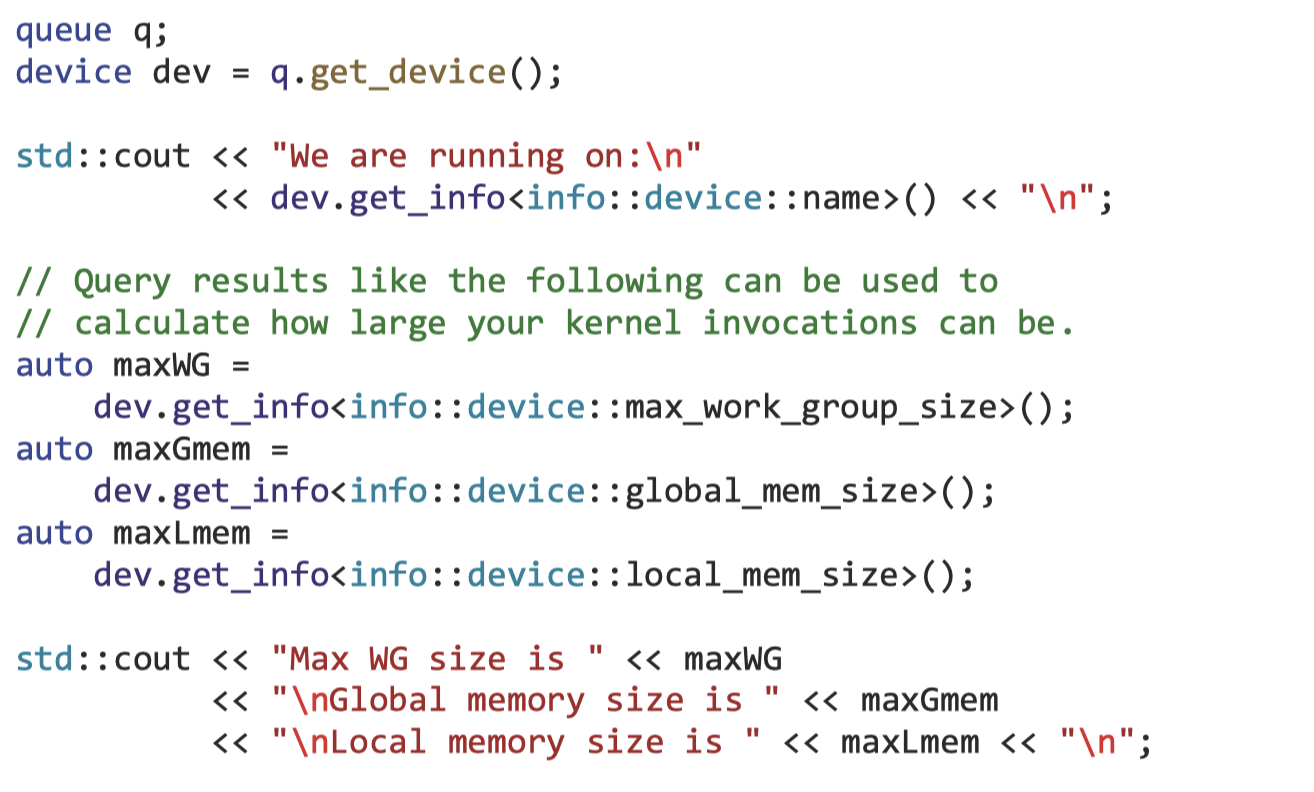
\includegraphics[width=0.9\textwidth]{figs/F12.8.png}
	\caption{\textit{线程 1 的 co-rank 函数操作示例的迭代 2。}}
\end{figure}

在迭代 2 期间,如图 12.8 所示,$\mathrm{i}$ 和 $\mathrm{j}$ 值为 2 和 1。
两个 if 结构(第 9 行和第 14 行)都会找到 $\mathrm{i}$ 和 $\mathrm{j}$ 值可接受。 
对于第一个 if 构造, $\mathrm{A}[\mathrm{i}-1]$ 是 $\mathrm{A}[1]$ (值 7 )和 $\mathrm{B}[\mathrm{j}] $ 是 $\mathrm{B}[1]$ (值 10),因此满足条件 $A[i-1] \leq B[j]$。 
对于第二个 if 结构, $B[j-1]$ 是 $B[0]$ (值 7),$A$ [i] 是 $A[2]$ (值 8),所以条件 $B [j-1]<A[i]$ 也满足。 
co-rank 函数设置一个标志退出 while 循环(第 20 和 08 行)并返回最终的 $\mathrm{i}$ 值 2 作为 co-rank $\mathrm{i}$ 值(第 23 行) 。 
调用者线程可以将最终的联合秩 $\mathrm{j}$ 值导出为 $\mathrm{k}-\mathrm{i}=3-2=1$。 
对图 12.8 的检查证实,共同排序值 2 和 1 确实标识了线程 1 的正确 A 和 B 输入子数组。

读者应该对线程 2 重复相同的过程作为练习。 
另请注意,如果输入流更长,则每一步的增量值将减少一半,
因此算法的复杂度为 $\log _{2}(\mathrm{~N})$,其中 $\mathrm{N}$ 是两个输入数组大小中的最大值。

\subsection{一个基本的并行合并内核}
\begin{figure}[H]
	\centering
	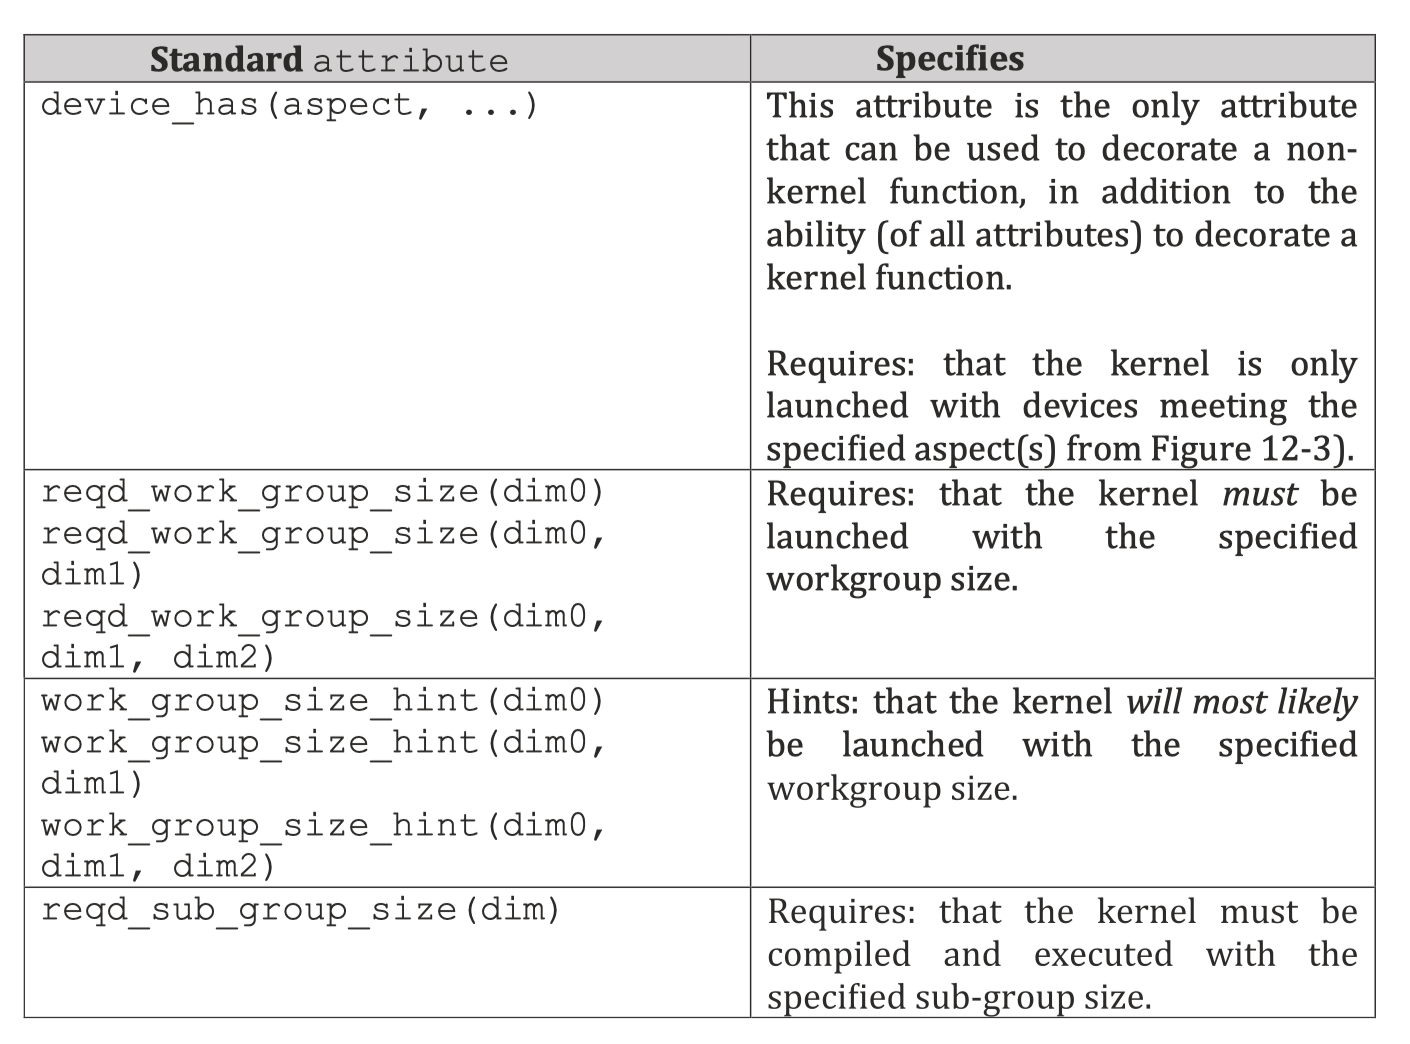
\includegraphics[width=0.9\textwidth]{figs/F12.9.png}
	\caption{\textit{一个基本的合并内核。}}
\end{figure}

在本章的其余部分中,我们假设输入 A 和 B 数组驻留在全局内存中。 
我们进一步假设启动一个内核来合并两个输入数组以生成一个输出数组 $\mathrm{C}$ ,该数组也位于全局内存中。 
图 12.9 显示了一个基本内核,它是第 12.3 节中描述的并行合并函数的直接实现。

正如我们所看到的,内核很简单。 
它首先通过计算当前线程 (k\_curr) 和下一个线程 (k\_next) 生成的输出子数组的起点来划分线程之间的工作。 
请记住,输出元素的总数可能不是线程数的倍数。 然后,每个线程对 co-rank 函数进行两次调用。
第一个调用使用 k\_curr 作为秩参数,它是当前线程要生成的输出子数组的第一个(最低索引)元素。 
返回的联合秩值 i\_curr 给出属于线程要使用的输入子数组的索引最低的输入数组元素。 
此联合秩值还可用于获取 $\mathrm{B}$ 输入子数组的 j\_curr。 i\_curr 和 j\_curr 值标记线程输入子数组的开头。 
因此 $\&\mathrm{~A}\left[\mathrm{i}_{-}\right.$curr] 
和 $\&\mathrm{~B}\left[\mathrm{j} \_\right .$curr $]$ 是指向当前线程要使用的输入子数组开头的指针。

第二次调用使用 k\_next 作为秩参数来获取下一个线程的共同秩值。 
这些共同秩值标记下一个线程要使用的最低索引输入数组元素的位置。 
因此 i\_next i\_curr 和 j\_next - j\_curr 给出了当前线程要使用的 A 和 B 子数组的大小。 
指向当前线程要生成的输出子数组开头的指针是 $\& C\left[\mathrm{k} \_\right.$curr $]$。 
内核的最后一步是使用这些参数调用 merge\_sequential 函数(来自图 12.2)。

基本合并内核的执行可以用图 12.8 中的例子来说明。 三个线程(线程 0,1 和 2 )的 k\_curr 值为 0 , 3 和 6。
我们将重点关注线程 1 的执行,其 $\mathrm{k}$ \_curr 值为 3 . 
从第一个 co-rank 函数调用确定的 i\_curr 和 j\_curr 值为 2 和 1 。 
线程 1 的 $\mathrm{k} \_$next 值为 6 。 
对 co-rank 函数的第二次调用有助于确定 5 和 1 的 i\_next 和 j\_next 值。 
然后线程 1 使用参数 (\&A[2], 3, \&B[1], 0, \& $\mathrm{C}[3])$ 调用合并函数。 
请注意,参数 $n$ 的值为 0 表示线程 1 的输出子数组的三个元素均不应来自数组 $\mathrm{B}$。 
这确实是图 12.8 中的情况:输出元素 $C[3]-C[5]$ 全部来自 $A[2]-A[4]$。 
虽然基本的合并内核非常简单和优雅,但它在内存访问效率方面存在不足。 
首先,很明显,当执行 merge\_sequential 函数时,
warp 中的相邻线程在读取和写入输入和输出子数组元素时不会访问相邻的内存位置。 
对于图 12.8 中的示例,在 merge\_sequential 函数执行的第一次迭代期间,
三个相邻线程将读取 $\mathrm{A}[0]、\mathrm{A}[2]$ 和 $\mathrm {B}[0]$。 
然后,它们将写入 $\mathrm{C}[0]、\mathrm{C}[3]$ 和 $\mathrm{C}[6]$。 
因此,它们的内存访问没有合并,导致内存带宽利用率不佳。

其次,线程在执行 co-rank 函数时还需要访问全局内存中的 A 和 B 元素。 
由于 co-rank 函数执行二分搜索,因此访问模式有些不规则,并且不太可能合并。 
结果,这些访问会进一步降低存储器带宽的利用效率。 
如果我们能够避免通过 co-rank 函数对全局内存进行这些未合并的访问,将会很有帮助。

\subsection{用于改进合并的平铺合并内核}
在第 6 章“性能注意事项”中,我们提到了改进内核内存合并的三种主要策略:
(1)重新安排线程到数据的映射,(2)重新安排数据本身,以及(3)在全局内存和全局内存之间传输数据。 
以合并的方式共享内存并在共享内存中执行不规则的访问。 对于合并模式,我们将使用第三种策略,该策略利用共享内存来改进合并。 
使用共享内存还具有捕获跨 co-rank 函数和顺序合并阶段的少量数据重用的优点。

关键的观察是相邻线程使用的输入 A 和 B 子数组在内存中彼此相邻。 
本质上,块中的所有线程将共同使用 A 和 B 的更大的块级子数组来生成 $\mathrm{C}$ 的更大的块级子数组。 
我们可以对整个块调用 co-rank 函数来获取块级 A 和 B 子数组的起始和结束位置。 
使用这些块级联合排序值,块中的所有线程可以以合并模式协作将块级 A 和 B 子数组的元素加载到共享内存中。

\begin{figure}[H]
	\centering
	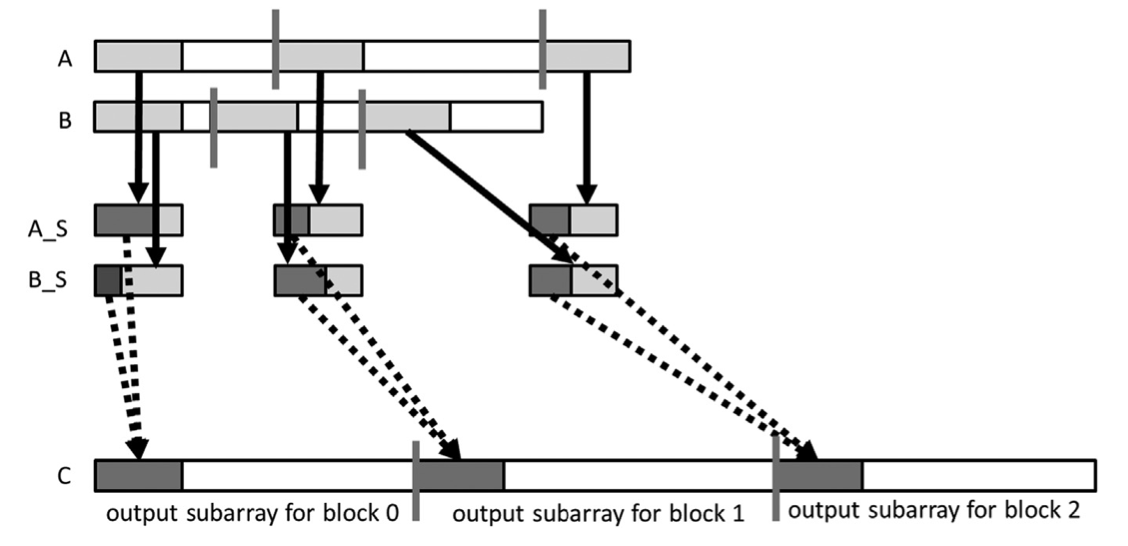
\includegraphics[width=0.9\textwidth]{figs/F12.10.png}
	\caption{\textit{平铺合并内核的设计。}}
\end{figure}

图 12.10 显示了平铺合并内核的块级设计。 在这个例子中,我们假设三个块将用于合并操作。 
在图的底部,我们显示 $\mathrm{C}$ 被划分为三个块级子数组。 我们用灰色竖条描绘这些分区。 
在分区的基础上,每个块调用 co-rank 函数将输入数组分区为每个块使用的子数组。 我们还用灰色竖条描绘输入分区。 
请注意,根据输入数组中的实际数据元素值,输入分区的大小可能会有很大差异。 
例如,在图 12.8 中,线程 0 的输入 A 子数组明显大于输入 B 子数组。 
另一方面,线程 1 的输入 A 子数组明显小于输入 B 子数组。
显然,两个输入子数组的组合大小必须始终等于每个线程的输出子数组的大小。

我们将为每个块声明两个共享内存数组 A\_S 和 B\_S。 
由于共享内存大小有限,A\_S 和 B\_S 可能无法覆盖该块的整个输入子数组。 
因此我们将采取迭代方法。 假设 A\_S 和 B\_S 数组各自可以容纳 x 个元素,而每个输出子数组包含 y 个元素。 
每个线程块将在 $y / x$ 迭代中执行其操作。 
在每次迭代期间,块中的所有线程将协作从块的输入 A 子数组中加载 $\mathrm{x}$ 元素,
并从其输入 B 子数组中加载 $\mathrm{x}$ 元素。

每个线程的第一次迭代如图 12.10 所示。 
我们表明,对于每个块,输入 A 子数组的浅灰色部分被加载到 A\_S 中,输入 B 子数组的浅灰色部分被加载到 B\_S 中。 
共享内存中有 x 个 A 元素和 $\mathrm{x} \mathrm{B}$ 元素,
线程块有足够的输入元素来生成至少 $\mathrm{x}$ 输出数组元素。 
所有线程都保证拥有迭代所需的所有输入子数组元素。 
有人可能会问为什么加载总共 $2 \mathrm{x}$ 输入元素可以保证仅生成 $\mathrm{x}$ 输出元素。 
原因是在最坏的情况下,当前输出部分的所有元素可能全部来自输入部分之一。 
输入使用的这种不确定性使得合并内核的平铺设计比以前的模式更具挑战性。 
通过首先调用当前和下一个输出部分的 co-rank 函数,可以更准确地加载输入图块。 
在这种情况下,我们付出额外的二分搜索操作来节省冗余数据加载。 我们将这种替代实现留作练习。 
我们还将在 12.7 节中通过循环缓冲区设计来提高内存带宽利用率。 
图 12.10 还显示,每个块中的线程将在每次迭代中使用 A\_S 的一部分和 B\_S 的一部分(显示为深灰色部分)
来生成 $\mathrm{x}$ 元素的部分 在其输出 $\mathrm{C}$ 子数组中。 
这个过程用从 A\_S 和 B\_S 深灰色部分到 C 深灰色部分的虚线箭头来说明。 
请注意,每个线程块很可能使用其 A\_S 与 B\_S 部分的不同部分。 
某些块可能会使用 A\_S 中的更多元素,而其他块可能会使用 B\_S 中的更多元素。 每个块使用的实际部分取决于输入数据元素值。

\begin{figure}[H]
	\centering
	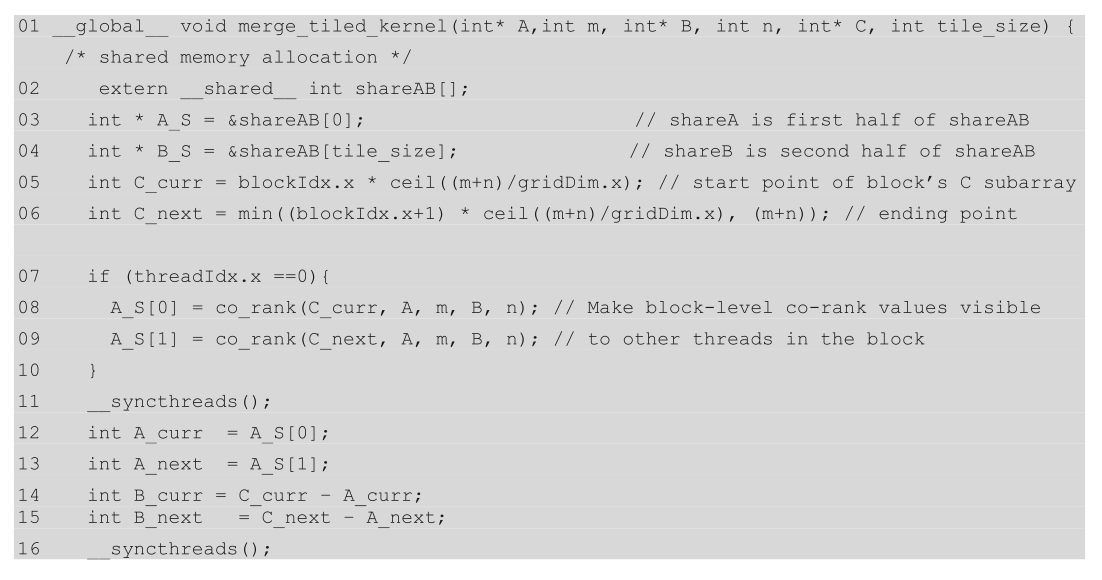
\includegraphics[width=0.9\textwidth]{figs/F12.11.png}
	\caption{\textit{第 1 部分:识别块级输出和输入子数组。}}
\end{figure}

图 12.11 显示了平铺合并内核的第一部分。 与图 12.9 的比较显示出显着的相似性。 
这部分本质上是线程级基本合并内核的设置代码的块级版本。 
块中只有一个线程需要计算当前块的开始输出索引的Rank值和下一个块的开始输出索引的Rank值。 
这些值被放置到共享内存中,以便块中的所有线程都可以看到它们。 
只有一个线程来调用 co-rank 函数减少了 co-rank 函数访问全局内存的次数,并且应该提高全局内存访问的效率。 
屏障同步用于确保所有线程都等待,直到共享内存 A\_S[0] 和 A\_S[1] 位置中的块级协同排序值可用,然后才继续使用这些值。

回想一下,由于输入子数组可能太大而无法放入共享内存,因此内核采用迭代方法。 
内核接收一个tile\_size参数,该参数指定共享内存中要容纳的$\mathrm{A}$元素和$\mathrm{B}$元素的数量。 
例如,tile\_size值为1024意味着共享存储器中要容纳1024个A数组元素和1024个B数组元素。 
这意味着每个块将专用 $(1024+1024) \times$ $4=8192$ 字节的共享内存来保存 A 和 B 数组元素。

举一个简单的例子,假设我们想要将包含 33,000 个元素的 A 数组 $(m=33,000)$ 
与包含 31,000 个元素的 B 数组 $(n=31,000)$ 合并。 输出 $C$ 元素的总数为 64,000 。 
进一步假设我们将使用 16 个块 (gridDim.x=16),每个块中使用 128 个线程 (blockDim.x=128)。 
每个块将生成 $64,000 / 16=4000$ 输出 $C$ 数组元素。

\begin{figure}[H]
	\centering
	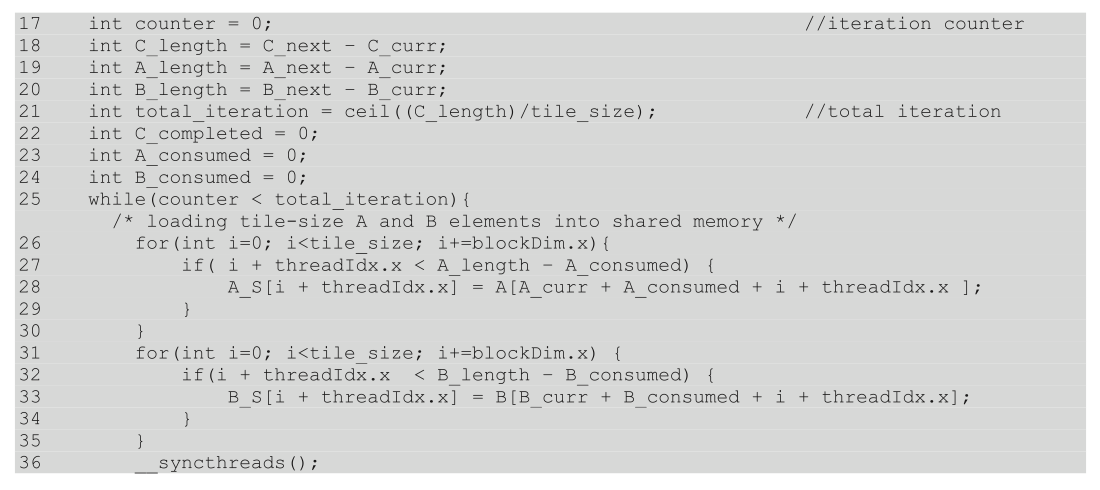
\includegraphics[width=0.9\textwidth]{figs/F12.12.png}
	\caption{\textit{第 2 部分:将 A 和 B 元素加载到共享内存中。}}
\end{figure}

如果我们假设tile\_size值为1024,则图12.12中的while循环将需要对每个块进行四次迭代才能完成其4000个输出元素的生成。 
在 while 循环的第 0 次迭代期间,每个块中的线程将协作将 A 的 1024 个元素和 B 的 1024 个元素加载到共享内存中。 
由于一个块中有 128 个线程,因此它们可以在 for 循环的每次迭代中总共加载 128 个元素(第 26 行)。 
因此,图12.12中的第一个for循环将为块中的所有线程迭代8次,以完成1024个A元素的加载。 
第二个 for 循环也将迭代 8 次以完成 $1024 \mathrm{~B}$ 元素的加载。 
请注意,线程使用其 threadIdx.x 值来选择要加载的元素,因此连续的线程会加载连续的元素。 
内存访问被合并。 我们稍后会解释 if 条件以及加载 A 和 B 元素的索引表达式是如何制定的。

\begin{figure}[H]
	\centering
	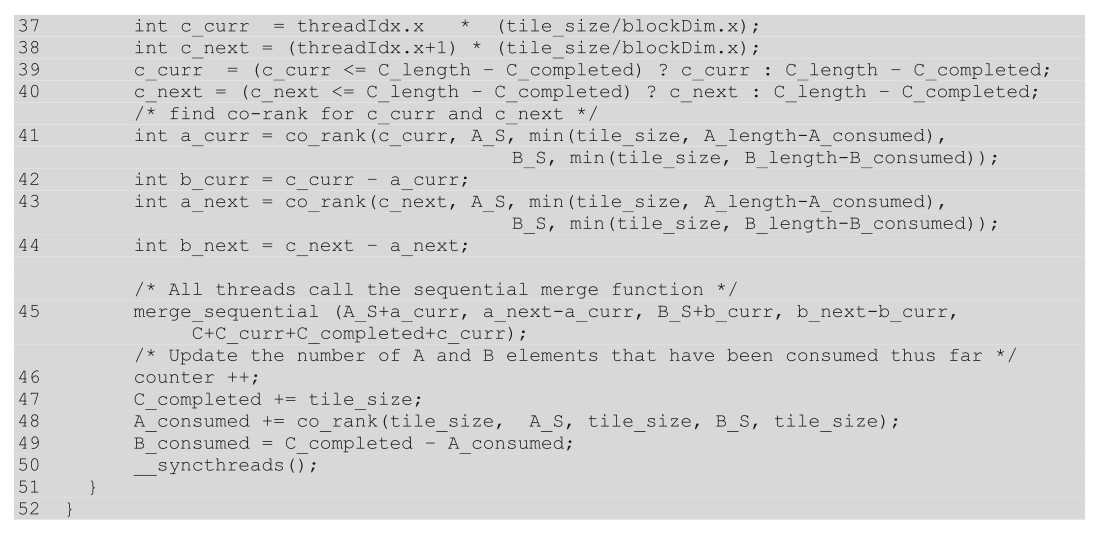
\includegraphics[width=0.9\textwidth]{figs/F12.13.png}
	\caption{\textit{第 3 部分:所有线程并行合并其各自的子数组。}}
\end{figure}

一旦输入图块位于共享内存中,各个线程就可以划分输入图块并并行合并它们的部分。 
这是通过将输出的一部分分配给每个线程并运行 co-rank 函数来确定应用于生成该输出部分的共享内存数据部分来完成的。 
图12.13中的代码完成了这一步。 请记住,这是图 12.12 中开始的 while 循环的延续。 
在 while 循环的每次迭代期间,块中的线程将使用我们加载到共享内存中的数据生成总共tile\_size $\mathrm{C}$ 元素。 
(最后一次迭代是个例外,这将在稍后解决。)co-rank 函数针对各个线程的共享内存中的数据运行。 
每个线程首先计算其输出范围和下一个线程的输出范围的起始位置,然后使用这些起始位置作为 co-rank 函数的输入来识别其输入范围。 
然后,每个线程将调用顺序合并函数,
将共享内存中的 $\mathrm{A}$ 和 B 元素部分(由 co-rank 值标识)合并到其指定的 $\mathrm{C}$ 元素范围中 。

让我们继续运行示例。 
在 while 循环的每次迭代中,块中的所有线程将使用共享内存中的 A 和 B 元素这两个输入块共同生成 1024 个输出元素。 
(稍后我们将再次处理 while 循环的最后一次迭代。)工作被分配给 128 个线程,因此每个线程将生成 8 个输出元素。 
虽然我们知道每个线程将消耗共享内存中总共八个输入元素,
但我们需要调用 co-rank 函数来找出每个线程将消耗的 A 元素与 B 元素的确切数量以及它们的开始和结束 地点。 
例如,一个线程可以使用三个A元素和五个B元素,而另一个线程可以使用六个A元素和两个B元素,等等。

在我们的示例中,块中所有线程用于迭代的 A 元素和 B 元素的总数总计为 1024。 
例如,如果一个块中的所有线程都使用 476 个 A 元素,我们知道它们还使用了 $1024-476=548$ B 元素。 
甚至有可能所有线程最终都使用 1024 个 A 元素和 0 个 B 元素。 请记住,共享内存中总共加载了 2048 个元素。 
因此,在 while 循环的每次迭代中,只有加载到共享内存中的 A 和 B 元素的一半会被块中的所有线程使用。

我们现在准备好检查核函数的更多细节。 
回想一下,我们跳过了用于将 $\mathrm{A}$ 和 $\mathrm{B}$ 元素从全局内存加载到共享内存的索引表达式的解释。 
对于 while 循环的每次迭代,加载 A 和 B 数组中当前图块的起始点取决于已消耗的 $\mathrm{A}$ 
和 $\mathrm{B}$ 元素的总数 while 循环的先前迭代期间块的所有线程。 
假设我们在变量 A\_consumed 中跟踪 while 循环的所有先前迭代所消耗的 A 元素的总数。 
在进入 while 循环之前,我们将 A\_consumed 初始化为 0。 
在 while 循环的迭代 0 期间,所有块都从 A[A\_curr] 开始其图块,因为 A\_consumed 在迭代 0 开始时为 0。 
在 while 循环的每次后续迭代期间,A 元素的图块将从 A[A\_curr + A\_consumed] 开始。

\begin{figure}[H]
	\centering
	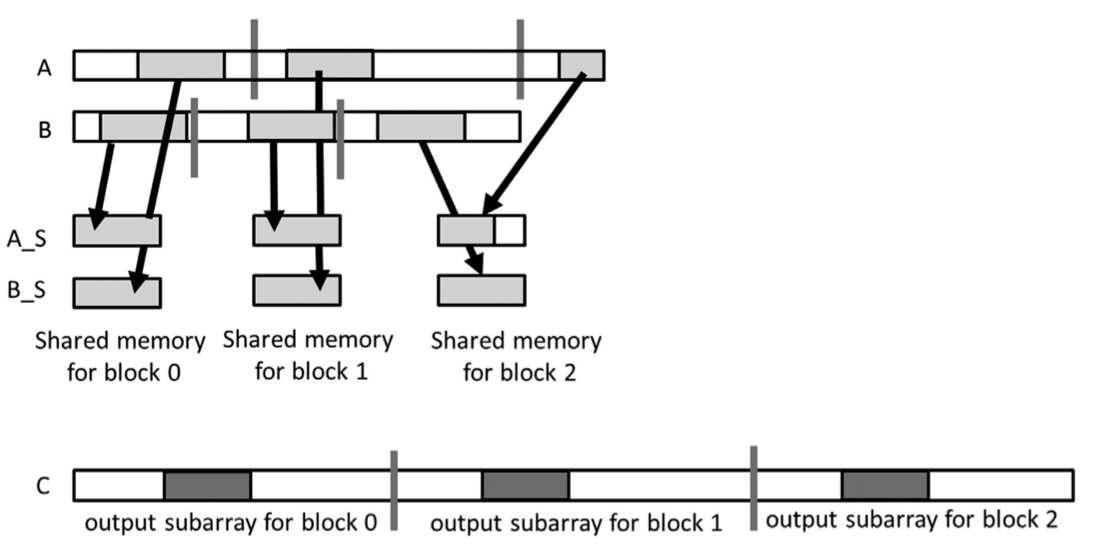
\includegraphics[width=0.9\textwidth]{figs/F12.14.png}
	\caption{\textit{运行示例中 while 循环的迭代 1。}}
\end{figure}

图 12.14 说明了 while 循环迭代 1 的索引计算。 
在图 12.10 的运行示例中,我们将迭代 0 期间线程块消耗的 A\_S 元素显示为 A\_S 中图块的深灰色部分。 
在迭代 1 期间,要从块 0 的全局内存加载的图块应从包含迭代 0 中消耗的 A 元素的部分之后的位置开始。
在图 12.14 中,对于每个块,A 元素的部分是 迭代 0 中消耗的内容显示为分配给该块的 A 子数组(由垂直条标记)开头的小白色部分。 
由于小部分的长度由 A\_consumed 的值给出,因此 while 循环的第 1 次迭代要加载的图块从 A[A\_curr + A\_consumed] 开始。 
类似地,要为 while 循环的迭代 1 加载的图块从 B[B\_curr + B\_consumed] 开始。

请注意,在图 12.13 中,A\_consumed(第 48 行)和 C\_completed 是通过 while 循环迭代累积的。 
此外,B\_consumed 是从累积的 A\_consumed 和 C\_completed 值得出的,因此它也是通过 while 循环迭代累积的。 
因此,它们始终反映迄今为止所有迭代消耗的 $\mathrm{A}$ 和 $\mathrm{B}$ 元素的数量。 
在每次迭代开始时,为迭代加载的图块始终以 A[A\_curr + A\_consumed] 和 B[B\_curr + B\_consumed] 开头。

在 while 循环的最后一次迭代期间,可能没有足够的输入 $\mathrm{A}$ 或 B 元素来填充某些线程块的共享内存中的输入图块。 
例如,在图 12.14 中,对于线程块 2,迭代 1 的剩余 A 元素的数量小于图块大小。 
应使用 if 语句来防止线程尝试加载块的输入子数组之外的元素。 
图 12.12(第 27 行)中的第一个 if 语句通过检查线程尝试加载的 A\_S 元素的索引是否超过表达式 A\ 的值给出的剩余 A 元素的数量来检测此类尝试。 \_length - A\_consumed。 if 语句确保线程仅加载 A 子数组剩余部分内的元素。 
B 元素也是如此(第 32 行)。

使用 if 语句和索引表达式,只要 A\_consumed 和 B\_consumed 给出了消耗的 $\mathrm{A}$ 和 $\mathrm{B}$ 元素的总数,
图块加载过程就应该正常工作。 while 循环的先前迭代中的线程块。 这将我们带到图 12.13 中 while 循环末尾的代码。 
这些语句更新迄今为止 while 循环迭代生成的 $\mathrm{C}$ 元素的总数。 
对于除最后一次迭代之外的所有迭代,每次迭代都会生成额外的tile\_size C 元素。

接下来的两个语句更新块中线程消耗的 A 和 B 元素的总数。 
对于除最后一次迭代之外的所有迭代,线程块消耗的附加 A 元素的数量是以下返回值

\begin{figure}[H]
	\centering
	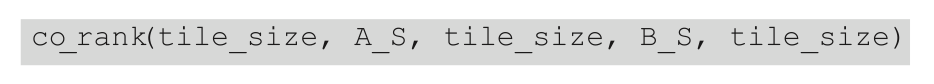
\includegraphics[width=0.9\textwidth]{figs/F12-a2.png}
\end{figure}

正如我们之前提到的,在 while 循环的最后一次迭代结束时消耗的元素数量的计算可能不正确。 
可能没有完整的元素可供最终迭代使用。 
但是,由于 while 循环不会进一步迭代,因此不会使用 A\_consumed、B\_consumed 和 C\_completed 值,
因此不正确的结果不会造成任何损害。 
但是,应该记住,如果出于某种原因在退出 while 循环后需要这些值,则这三个变量将不会具有正确的值。 
应改为使用 A\_length、B\_length 和 C\_length 的值,
因为线程块的指定子数组中的所有元素都将在 while 循环的出口处被消耗。

平铺内核通过 co-rank 函数实现了全局内存访问的大幅减少,并使全局内存访问合并。 
然而,事实上,内核有一个明显的缺陷。 它仅使用每次迭代中加载到共享内存中的一半数据。 
共享内存中未使用的数据只是在下一次迭代中重新加载。 这浪费了一半的内存带宽。 
在下一节中,我们将介绍一种循环缓冲区方案,用于管理共享内存中的数据元素块,
该方案允许内核充分利用已加载到共享内存中的所有 A 和 B 元素。 正如我们将看到的,效率的提高伴随着代码复杂性的大幅增加。

\subsection{循环缓冲区合并内核}
循环缓冲区合并内核(称为 merge\_circular\_buffer\_kernel)的设计与上一节中的 merge\_tiled\_kernel 内核的设计基本相同。 
主要区别在于共享内存中 $\mathrm{A}$ 和 $\mathrm{B}$ 元素的管理,以充分利用从全局内存加载的所有元素。 
merge\_tiled\_内核的整体结构如图 12.12 至 12.14 所示; 
它假设 A 和 B 元素的图块始终分别从 A\_S[0] 和 B\_S[0] 开始。 
在每次 while 循环迭代之后,内核加载下一个图块,从 A\_S[0] 和 B\_S [0] 开始。 
merge\_tiled\_kernel 的低效率源于这样一个事实:接下来的部分元素位于共享内存中,
但我们从全局内存中重新加载整个图块,并覆盖上一次迭代中的剩余元素。

\begin{figure}[H]
	\centering
	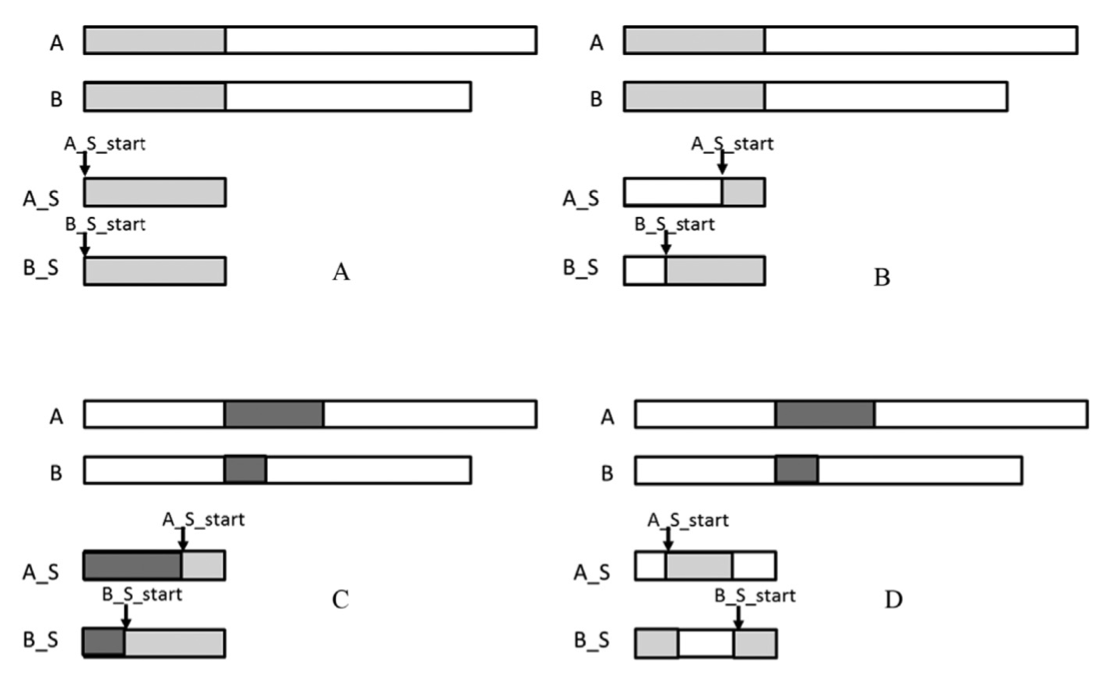
\includegraphics[width=0.9\textwidth]{figs/F12.15.png}
	\caption{\textit{用于管理共享内存块的循环缓冲区方案。}}
\end{figure}

图12.15展示了merge\_circular\_buffer\_kernel的主要思想。 我们将继续使用图 12.10 和 12.14 中的示例。 
添加两个附加变量 A\_S\_start 和 B\_S\_start,
以允许图 12.12 中 while 循环的每次迭代在 A\_S[0] 内动态确定的位置处启动其 A 和 B 块,
并且 分别为 B\_S[0]。 添加的跟踪允许 while 循环的每次迭代都使用上一次迭代中剩余的 A 和 B 元素来启动图块。 
由于第一次进入 while 循环时没有之前的迭代,因此这两个变量在进入 while 循环之前被初始化为 0。

在迭代 0 期间,由于 A\_S\_start 和 B\_S\_start 的值均为 0,因此图块将以 A\_S[0] 和 B\_S[0] 开始。 
这如图 12.15A 所示,其中我们将将从全局内存(A 和 B)加载到共享内存(A\_S 和 B\_S)中的图块显示为浅灰色部分。 
一旦这些tiles被加载到共享内存中,merge\_circular\_buffer\_kernel 
将以与 merge\_tile\_kernel 相同的方式继续进行合并操作。

我们还需要更新 A\_S\_start 和 B\_S\_start 变量,以便在下一次迭代中使用,
方法是将这些变量的值增加从共享内存消耗的 $\mathrm{A}$ 和 B 元素的数量 在当前迭代期间。 
请记住,每个缓冲区的大小仅限于tile\_size。 在某些时候,我们需要重用 A\_S 和 B\_S 数组开头部分的缓冲区位置。 
这是通过检查新的 A\_S\_start 和 B\_S\_start 值是否超过图块大小来完成的。 
如果是这样,我们从它们中减去tile\_size,如以下if语句所示:

\begin{figure}[H]
	\centering
	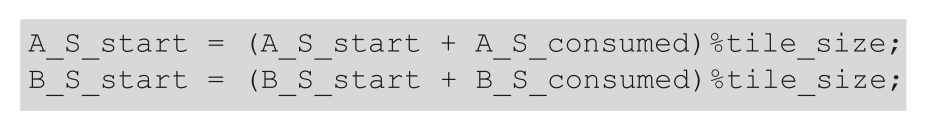
\includegraphics[width=0.9\textwidth]{figs/F12-a3.png}
\end{figure}

图12.15B说明了A\_S\_start和B\_S\_start变量的更新。 
在迭代 0 结束时,$\mathrm{A}$ 图块的一部分和 $\mathrm{B}$ 图块的一部分已被消耗。 
消耗的部分在图 12.15B 中的 A\_S 和 B\_S 中显示为白色部分。 
我们将 A\_S\_start 和 B\_S\_start 值更新到紧接在共享内存中已消耗部分之后的位置。

图 $12.15 \mathrm{C}$ 说明了在 while 循环的迭代 1 开始时填充 $\mathrm{A}$ 和 $\mathrm{B}$ 块的操作。 
A\_S\_consumed 是一个变量,添加它是为了跟踪当前迭代中使用的 $\mathrm{A}$ 元素的数量。 
该变量对于在下一次迭代中填充图块很有用。 
在每次迭代开始时,我们需要加载最多 A\_S\_consumed 元素的一部分,以填充共享内存中的 A 瓦片。 
类似地,我们需要加载一段最多 B\_S\_consumed 元素来填充共享内存中的 B 块。 
加载的两个部分在图 12.15C 中显示为深灰色部分。 
请注意,图块实际上在 A\_S 和 B\_S 数组中“环绕”,
因为我们正在重用在迭代 0 期间消耗的 $\mathrm{A}$ 和 $\mathrm{B}$ 元素的空间 。

图12.15D说明了在迭代1结束时对A\_S\_start和B\_S\_start的更新。 迭代 1 期间消耗的元素部分显示为白色部分。 
请注意,在 A\_S 中,消耗的部分会回绕到 A\_S 的开头部分。 A\_S\_start 变量的值也由 \% 模运算符包裹。 
应该清楚的是,我们需要调整加载和使用平铺元素的代码以支持 A\_S 和 B\_S 数组的循环使用。

\begin{figure}[H]
	\centering
	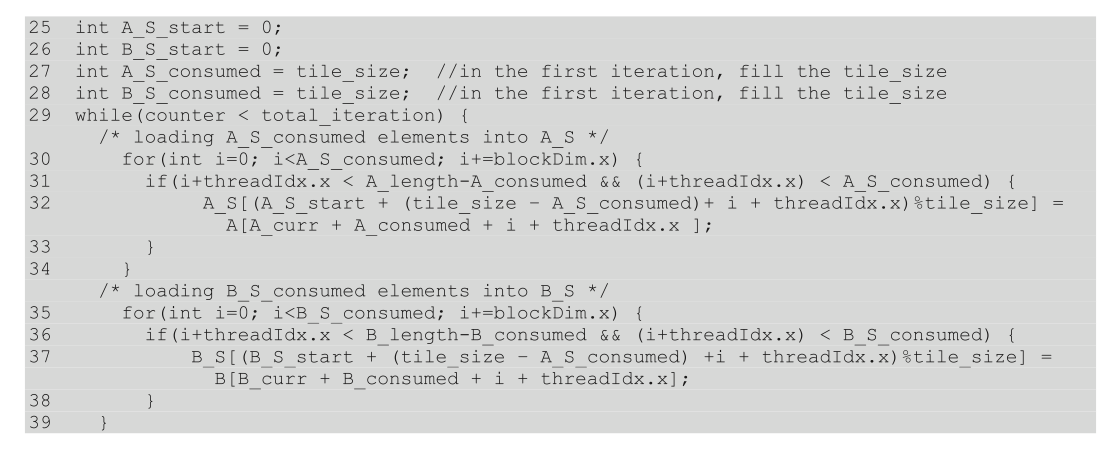
\includegraphics[width=0.9\textwidth]{figs/F12.16.png}
	\caption{\textit{循环缓冲区合并内核的第 2 部分。}}
\end{figure}

merge\_circular\_buffer\_kernel 的第 1 部分与图 12.11 中的 merge\_tiled\_kernel 相同,因此我们不再介绍它。 
图 12.16 显示了循环缓冲区内核的第二部分。 请参阅图 12.12,了解保持不变的变量声明。 
新变量 A\_S\_start、B\_S\_start、A\_S\_consumed 和 B\_S\_consumed 在进入 while 循环之前被初始化为 0。

请注意,两个 for 循环的退出条件已被调整。 与图 12.12 中的合并内核中的情况不同,
图 12.16 中的每个 for 循环都设置为仅加载重新填充图块所需的元素数量,而不是始终加载完整图块,由 A 给出 \_S\_消耗了。 
在第 i 个 for 循环迭代中由线程块加载的 A 元素部分从全局内存位置 A[A\_curr + A\_consumed + i] 开始。 
请注意,每次迭代后 $i$ 都会增加 blockDim.x。 
因此,第 i 个 forloop 迭代中线程要加载的 A 元素是 A[A\_curr + A\_consumed $+\mathrm{i}+$ threadIdx.x]。 
每个线程将其 A 元素放入 A\_S 数组的索引为 A\_S\_start + (tile\_size A\_S\_consumed $)+$ I + threadIdx,
因为图块从 A\_S[A 开始 \_S\_start] 并且在 while 循环的上一次迭代中,
缓冲区中剩余 (tile\_size - A\_S\_consumed) 个元素。 取模(\%)运算检查索引值是否大于或等于tile\_size。 
如果是,则通过从索引值中减去tile\_size 将其重新包装回数组的开头部分。 
相同的分析适用于加载 B 图块的 for 循环,并留给读者作为练习。

\begin{figure}[H]
	\centering
	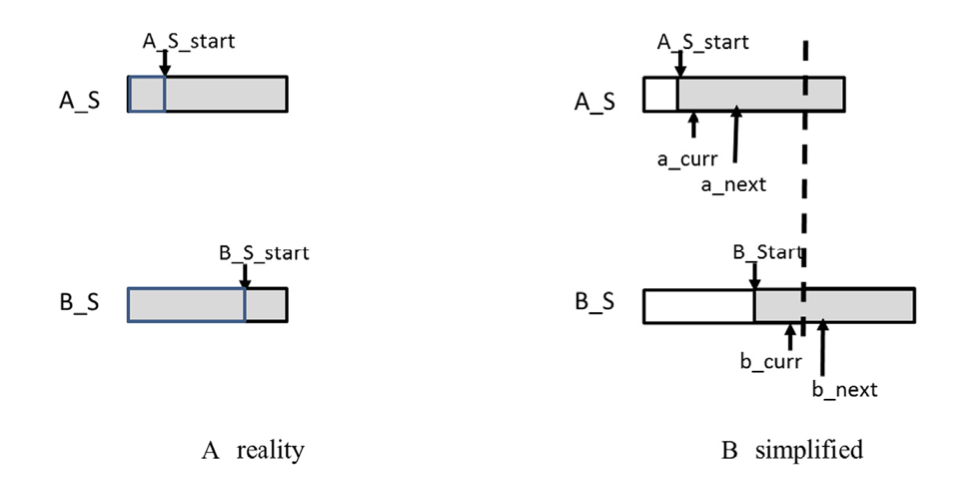
\includegraphics[width=0.9\textwidth]{figs/F12.17.png}
	\caption{\textit{使用循环缓冲区时联合排名值的简化模型。}}
\end{figure}

使用 A\_S 和 B\_S 数组作为循环缓冲区也会在实现 co-rank 和 merge 函数时带来额外的复杂性。 
部分额外的复杂性可能反映在调用这些函数的线程级代码中。 
然而,一般来说,如果能够有效地处理库函数内部的复杂性,以最大限度地减少用户代码中增加的复杂性,那就更好了。 
我们在图 12.17 中展示了这种方法。 图 12.17A 显示了循环缓冲区的实现。 
A\_S\_start 和 B\_S\_start 标记循环缓冲区中图块的开始。 
这些图块环绕在 A\_S 和 B\_S 数组中,如 A\_S\_start 和 B\_S\_start 左侧的浅灰色部分所示。

请记住,线程使用共同秩值来标识它们要使用的输入子数组的起始位置、结束位置和长度。 
当我们使用循环缓冲区时,我们可以提供联合秩值作为循环缓冲区中的实际索引。 
然而,这会导致 merge\_circular\_buffer\_kernel 代码变得相当复杂。 
例如,a\_next 值可能小于 a\_curr 值,因为图块环绕在 A\_S 数组中。 
因此,需要测试这种情况并将该部分的长度计算为 a\_next-a\_curr +tile\_size。 
然而,在其他情况下,当 a\_next 大于 a\_curr 时,该部分的长度只是 a\_next - a\_curr。

图 12.17B 显示了用于定义、导出和使用具有循环缓冲区的共同排序值的简化模型。 
在此模型中,每个图块似乎位于从 A\_S\_start 和 B\_S\_start 开始的连续部分中。 
在图 12.17A 中的 B\_S 图块的情况下,b\_next 被环绕并且将小于循环缓冲区中的 b\_curr。 
然而,如图12.17B所示,简化模型提供了一种错觉,即所有元素都位于最多tile\_size元素的连续部分中; 
因此,a\_next 始终大于或等于 a\_curr,而 b\_next 始终大于或等于 b\_curr。 
由 co\_rank\_circular 和 merge\_sequential\_circular 函数的实现
来将 corank 值的简化视图映射到实际的循环缓冲区索引中,以便它们能够正确有效地执行其功能。

\begin{figure}[H]
	\centering
	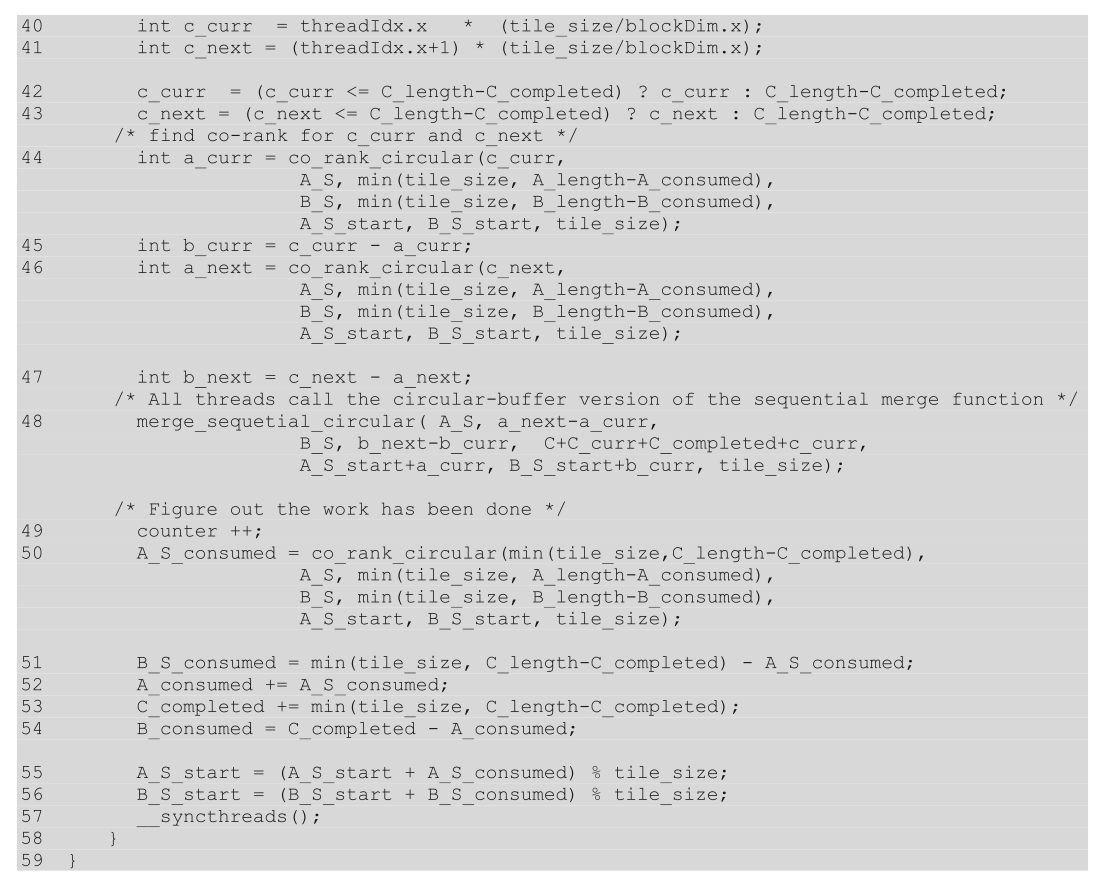
\includegraphics[width=0.9\textwidth]{figs/F12.18.png}
	\caption{\textit{循环缓冲区合并内核的第 3 部分。}}
\end{figure}

co\_rank\_circular 和 merge\_sequential\_circular 函数具有与原始 co\_rank 和 merge 函数相同的参数集,
外加三个附加参数:A\_S\_start、B\_S\_start 和tile\_size。 
这三个附加参数通知函数缓冲区的当前起点在哪里以及缓冲区有多大。 
图 12.18 显示了基于使用循环缓冲区的 co-rank 值的简化模型的修订后的线程级代码。 
代码的唯一更改是调用 co\_rank\_circular 和 merge\_sequential\_circular 函数,而不是 co\_rank 和 merge 函数。 
这表明,设计良好的库接口可以减少使用复杂数据结构时对用户代码的影响。

\begin{figure}[H]
	\centering
	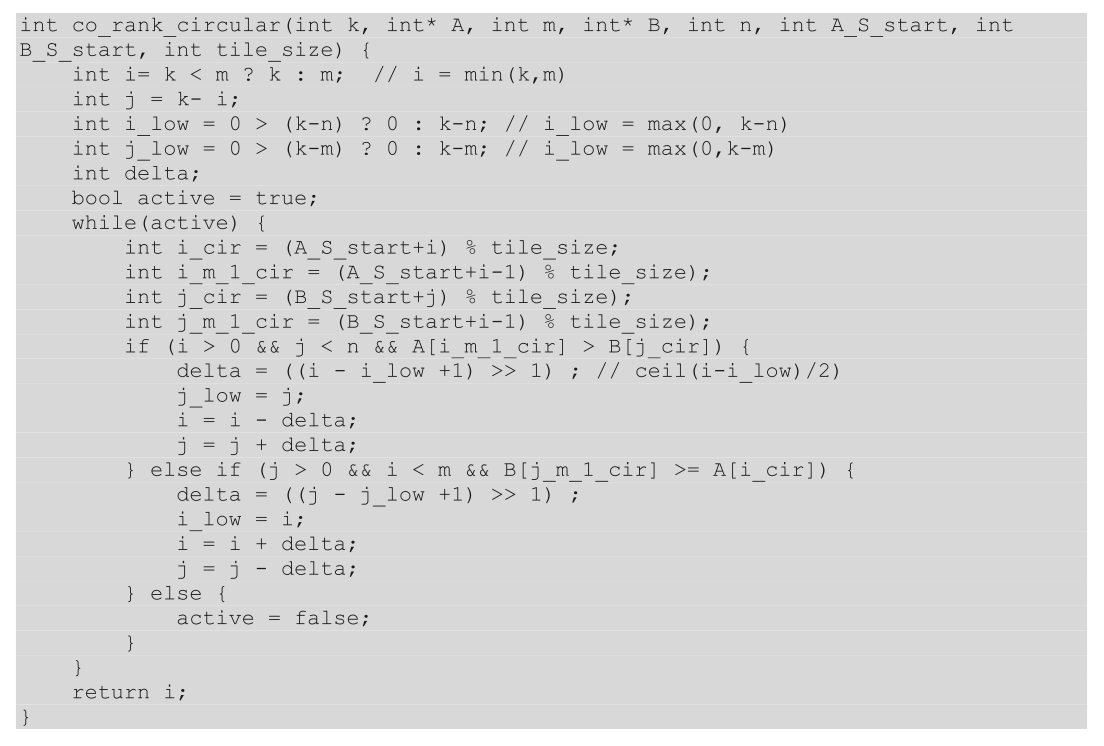
\includegraphics[width=0.9\textwidth]{figs/F12.19.png}
	\caption{\textit{在循环缓冲区上运行的 co\_rank\_circular 函数。}}
\end{figure}

图 12.19 显示了 co-rank 函数的实现,它提供了 co-rank 值的简化模型,同时在循环缓冲区上正确运行。 
它处理 i、j、i\_low 和 j\_low 值的方式与图 12.5 中的 co-rank 函数完全相同。 
唯一的变化是 i、i - 1、j 和 j - 1 不再直接用作访问 A\_S 和 B\_S 数组的索引。 
它们用作要添加到 A\_S\_start 和 B\_S\_start 的值的偏移量,
以形成索引值 i\_cir、i\_m\_1\_cir、j\_cir 和 j\_m\_1\_cir。 
在每种情况下,我们都需要测试实际索引值是否需要回绕到缓冲区的开始部分。 
请注意,我们不能简单地使用 i\_cir - 1 来替换 i - 1。我们需要形成最终的索引值并检查是否需要将其环绕。 
应该清楚的是,简化模型还有助于保持 co-rank 函数代码简单:i、j、i\_low 和 j\_low 值的所有操作保持不变; 
他们不需要处理缓冲区的循环性质。

\begin{figure}[H]
	\centering
	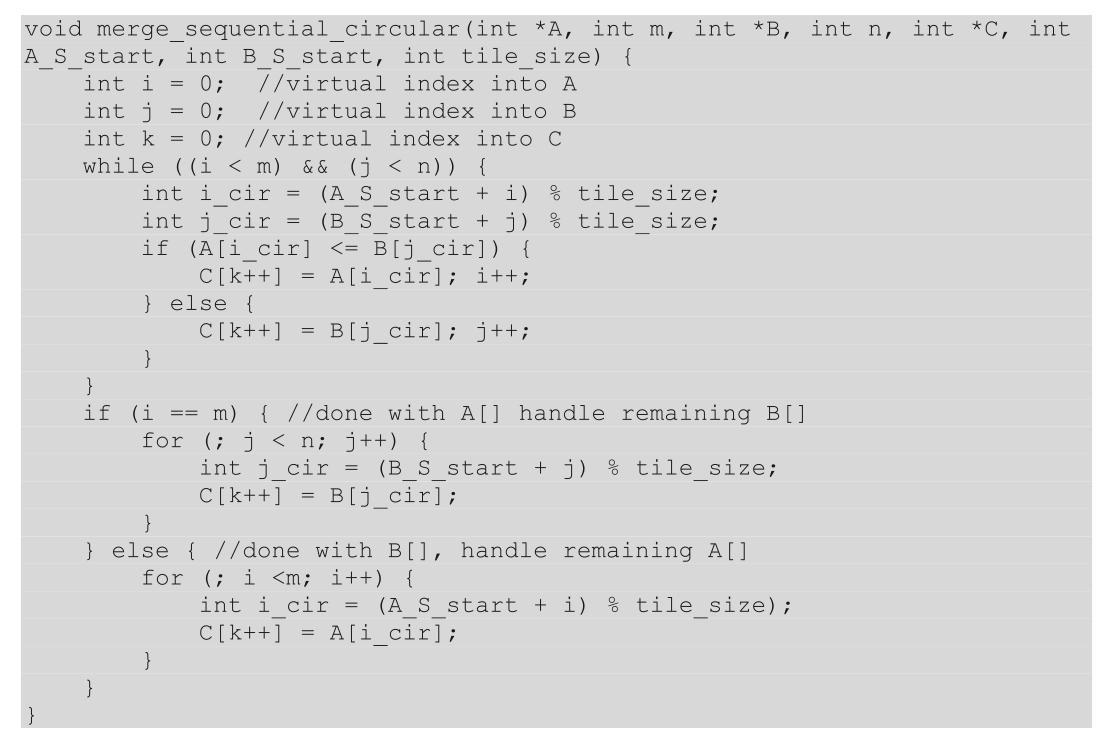
\includegraphics[width=0.9\textwidth]{figs/F12.20.png}
	\caption{\textit{merge\_sequential\_circular 函数的实现。}}
\end{figure}

图 12.20 显示了 merge\_sequential\_circular 函数的实现。 
与 co\_rank\_circular 函数类似,代码逻辑与原始合并函数基本保持不变。 
唯一的变化是使用 i 和 j 访问 A 和 B 元素的方式。 
由于merge\_sequential\_circular函数只会被merge\_circular\_buffer\_kernel的线程级代码调用,
因此访问的A和B元素将位于A\_S和B\_S数组中。 
在使用 i 或 j 访问 A 或 B 元素的所有四个地方,我们需要形成 i\_cir 或 j\_cir 并测试索引值是否需要绕回数组的开头部分。 
除此之外,代码与图 12.2 中的合并函数相同。

虽然我们没有列出 merge\_circular\_buffer\_kernel 的所有部分,但读者应该能够根据我们讨论的部分将它们放在一起。 
平铺和循环缓冲区的使用增加了相当多的复杂性。 特别是,每个线程使用更多的寄存器来跟踪起点和缓冲区中的剩余元素数量。 
所有这些额外的使用都可能会减少占用率,或者在执行内核时可以分配给每个流式多处理器的线程块的数量。 
然而,由于合并操作受内存带宽限制,因此计算资源和寄存器资源可能未得到充分利用。 
因此,增加所使用的寄存器的数量和地址计算以节省内存带宽是一个合理的权衡。

\subsection{合并的线程粗化}
跨多个线程并行合并的代价主要是每个线程必须执行自己的二分搜索操作来识别其输出索引的 Corrank。 
可以通过减少启动的线程数量来减少所执行的二分搜索操作的数量,这可以通过为每个线程分配更多输出元素来完成。 
本章中介绍的所有内核都已经应用了线程粗化,因为它们都是为每个线程处理多个元素而编写的。 
在完全未粗化的内核中,每个线程将负责单个输出元素。 然而,这需要对每个元素执行二分搜索操作,这将是非常昂贵的。 
因此,粗化对于分摊大量元素的二分搜索操作的成本至关重要。

\subsection{总结}
在本章中,我们介绍了有序合并模式,其并行化要求每个线程动态识别其输入位置范围。 
由于输入范围与数据相关,因此我们采用 co-rank 函数的快速搜索实现来识别每个线程的输入范围。 
当我们使用平铺技术来节省内存带宽并启用内存合并时,输入范围依赖于数据的事实也带来了额外的挑战。 
因此,我们引入了循环缓冲区的使用,以允许我们充分利用从全局内存加载的数据。 
我们表明,引入更复杂的数据结构(例如循环缓冲区)可以显着增加使用该数据结构的代码的复杂性。 
因此,我们为操作和使用索引的代码引入了一个简化的缓冲区访问模型,以保持基本不变。 
仅当这些索引用于访问缓冲区中的元素时,缓冲区的实际循环性质才会暴露。